\chapter{Appendix 3}
\lhead{\textit{Appendix 3}}
This appendix contains the data analysis (using Python) for the analysis described in Chapter 5. For this corpus, recordings were collected consisting of audio and video representing different perspectives on mining and natural resource development. Below are the segments analysed as well as links to the original media.


Raw data and analysis is available in the folder \textit{Analysis 3} in a GitHub repo: \href{https://github.com/craigmateo/multilevel_corpus}{https://github.com/craigmateo/multilevel\_corpus}

\section{Annotation Scheme}

\begin{table}[H]
\begin{footnotesize}
\centering
\def\arraystretch{.9}% 
\begin{tabular}{ | P{2cm} P{3cm} P{6cm}|}  
\hline
(.)             & Micro-pause                    & A brief pause, usually less than 0.2 seconds.                                                                      \\ \hline
. or down arrow & Period or Down Arrow           & Indicates falling pitch or intonation.                                                                             \\ \hline
? or up arrow   & Question Mark or Up Arrow      & Indicates rising pitch or intonation.                                                                              \\ \hline
,               & Comma                          & Indicates a temporary rise or fall in intonation.                                                                  \\ \hline
!-              & Hyphen                         & Indicates an abrupt halt or interruption in utterance.                                                             \\ \hline
>text<          & Greater than/Less than symbols & Indicates that the enclosed speech was delivered more rapidly than usual for the speaker.                          \\ \hline
<text>          & Less than/Greater than symbols & Indicates that the enclosed speech was delivered more slowly than usual for the speaker.                          \\ \hline
\degree         & Degree symbol                  & Indicates whisper, reduced volume or quiet speech.                                                                 \\ \hline
ALL CAPS        & Capitalized text               & Indicates shouted or increased-volume speech                                                                       \\ \hline
underline       & Underlined text                & Indicates the speaker is emphasising or stressing the speech.                                                      \\ \hline
:::             & Colon(s)                       & Indicates prolongation of a sound.                                                                                 \\ \hline
hhh             &                                & Audible exhalation                                                                                                 \\ \hline
.hhh            &                                & Audible inhalation                                                                                                 \\ \hline
(text)          & Parentheses                    & Speech which is unclear or in doubt in the transcript.                                                             \\ \hline
[text]          & Square brackets                & Speech within square brackets is accompanied by the meaningful part of the gesture - the so-called `stroke phase'. \\ \hline
\end{tabular}
\caption{Gail Jefferson's (\citeyear{Jefferson2004}) annotation scheme \\ as adapted by \cite[5]{Beattie2016}. }
\label{tab:table1}
\end{footnotesize}
\end{table}



\section{Ecological-Level}

\subsection{Ecological Level - Example 1}

\begin{footnotesize}

Source: \url{https://www.youtube.com/embed/-UPjsuuyvD4?start=632&end=653}\\
\textit{Embeded videos require Adobe Flash.}
\begin{center}
\includemedia[width=9.60cm,height=5.40cm,activate=pageopen,
passcontext,
transparent,
addresource=Figures/05.mp4,
flashvars={source=Figures/05.mp4}
]{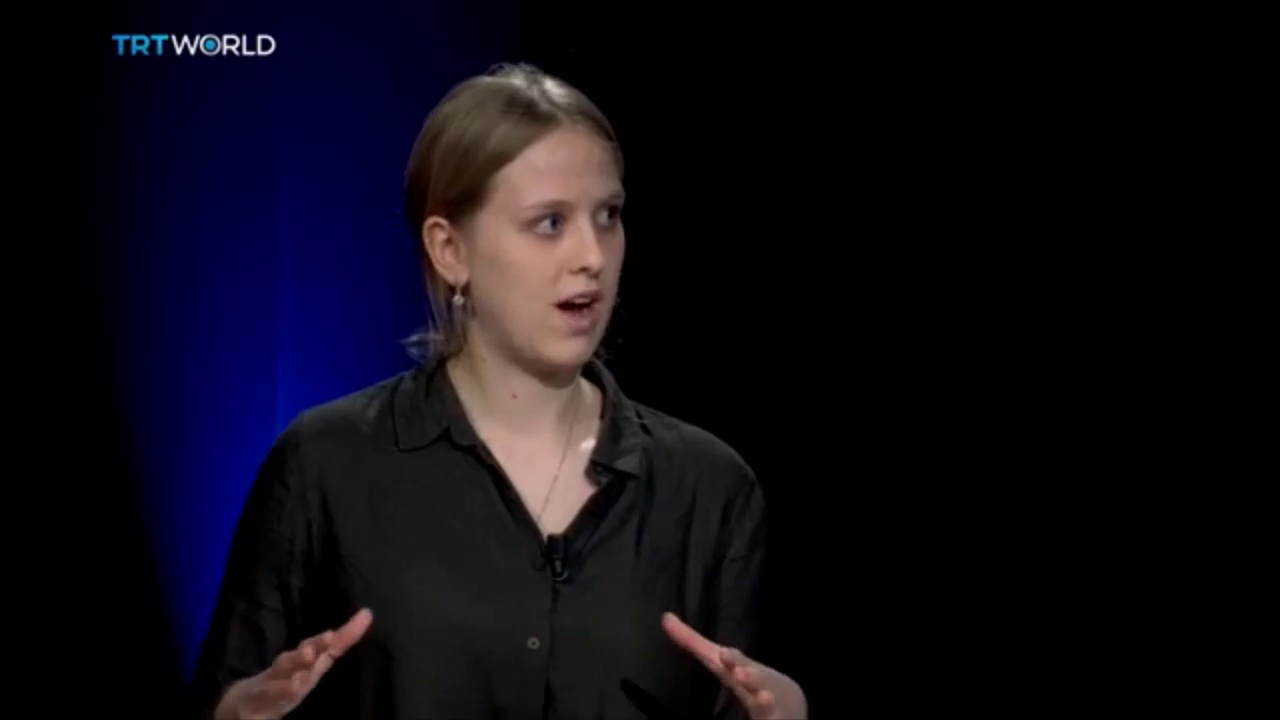
\includegraphics{Figures/play1.png}}{VPlayer.swf}
\end{center}

\texttt{[the] \annotate{direct impact}\textsuperscript{1} will likely result in biodiversity loss that will be very difficult to \annotate{recover from}\textsuperscript{2} but we really don't understand is any of the \annotate{wider impacts}\textsuperscript{3} as well, so outside the \annotate{area of}\textsuperscript{4} mining itself how will this \annotate{affect the ecosystem at large how will this feedback into the oceans}\textsuperscript{5} we think that the deep sea...}

\end{footnotesize}

\begin{footnotesize}
\begin{enumerate}
   \item HAND downward in swift movement, fingers pointed outward
   \item HANDS in cycling motion forward
   \item HANDS expanding outwards
   \item HAND in wide circular movement with palm down
   \item HANDS in cycling movement with palms inwards
\end{enumerate}
\end{footnotesize}

\begin{figure}[H]
\centering
\begin{tabular}{llll}
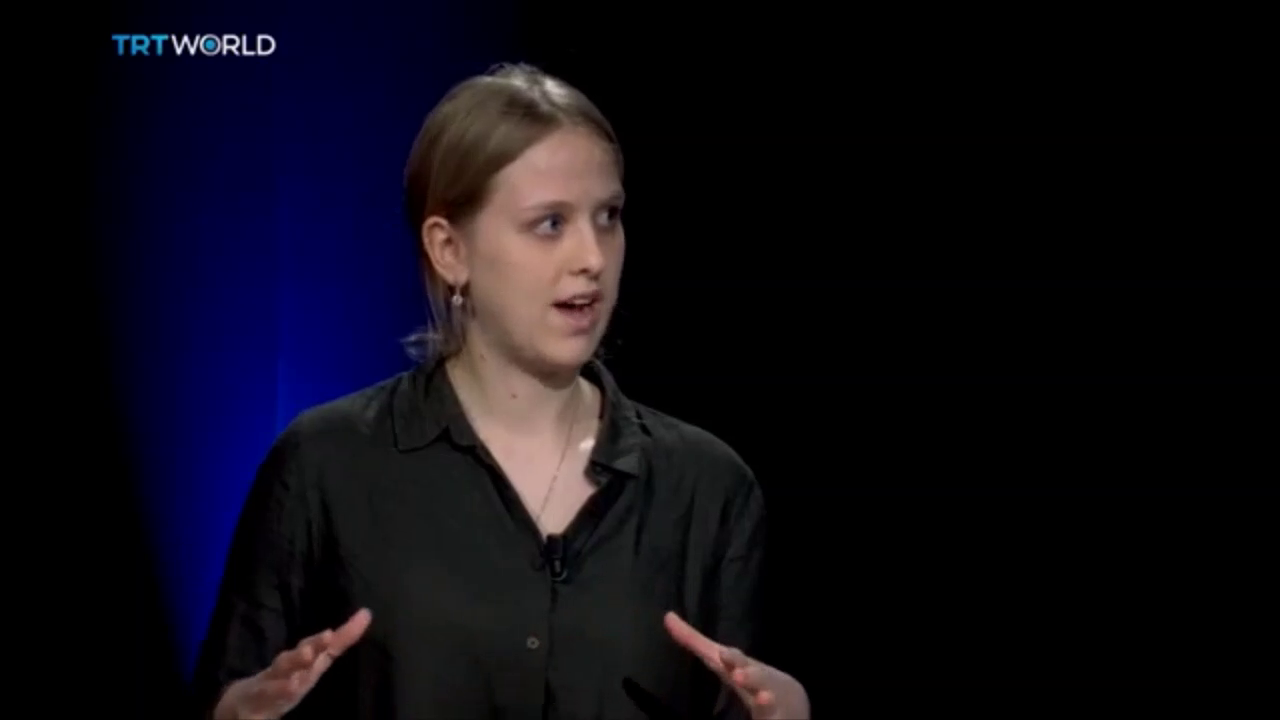
\includegraphics[width=4.2cm]{Figures/mmEco/frame207.png} & 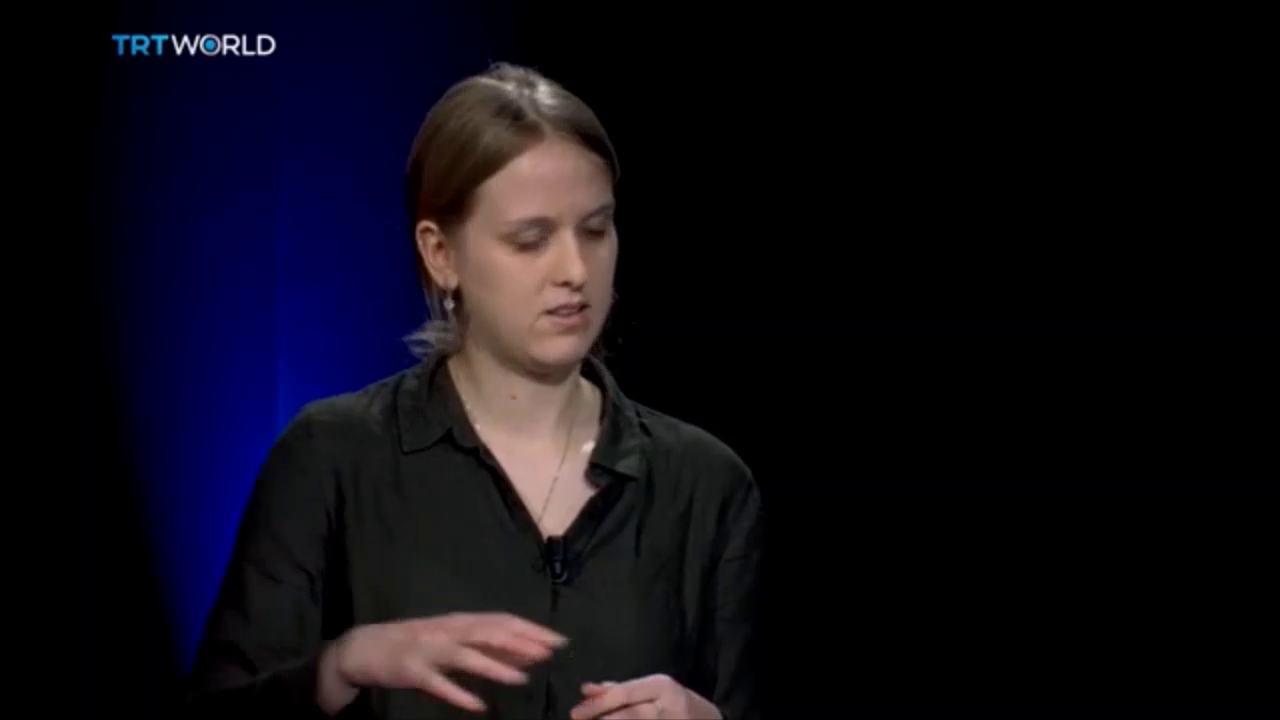
\includegraphics[width=4.2cm]{Figures/mmEco/frame252.png} & 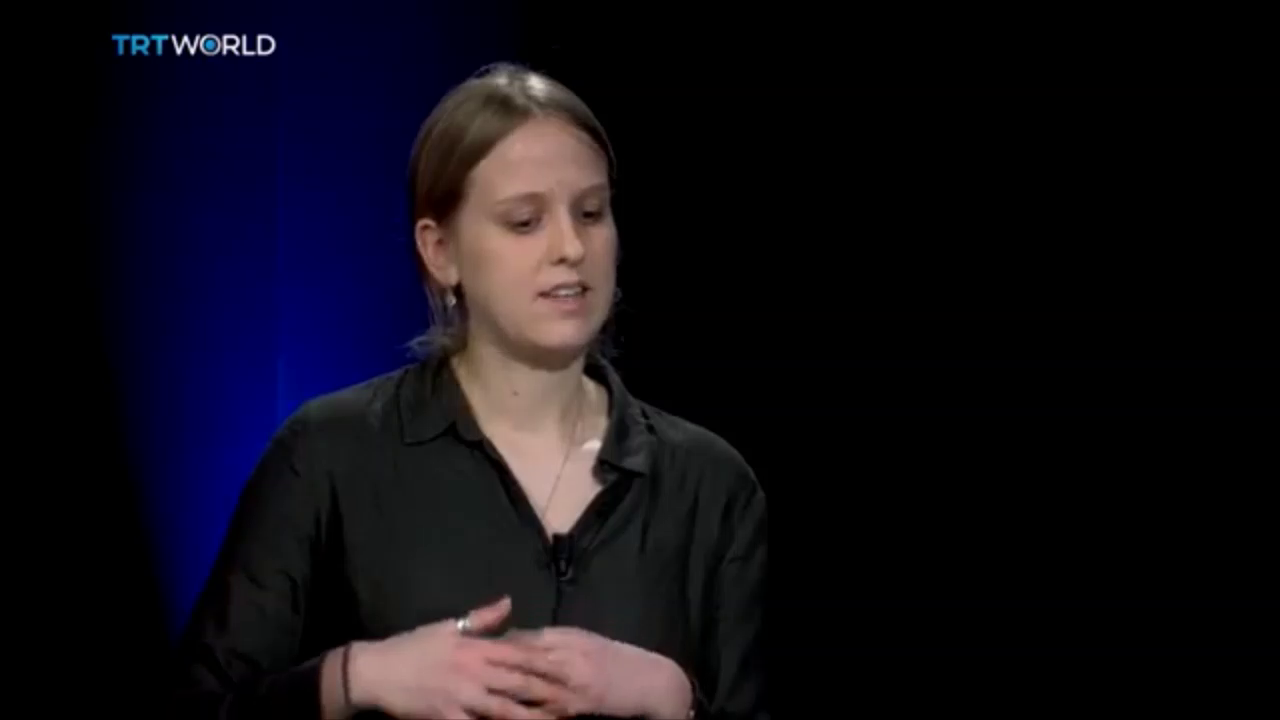
\includegraphics[width=4.2cm]{Figures/mmEco/frame392.png} 

\end{tabular}
\caption{Ecological Level - Example 1}

\begin{footnotesize}
Left: hands open palms down gesture with fingers extended to emphasize direct ecological impacts. Middle, Right: Hands loosened, palms inward/down in a cycling motion to reflect less certain long term ecological processes and feedback mechanisms.


\end{footnotesize}



\label{fig:figure1}
\end{figure}

\subsection{Ecological Level - Example 2}

\begin{footnotesize}
Source: \url{https://www.youtube.com/embed/Sh0_Wf8F4RM?start=857&end=888)}\\
\textit{Embeded videos require Adobe Flash.}
\begin{center}
\includemedia[width=9.60cm,height=5.40cm,activate=pageopen,
passcontext,
transparent,
addresource=Figures/10.mp4,
flashvars={source=Figures/10.mp4}
]{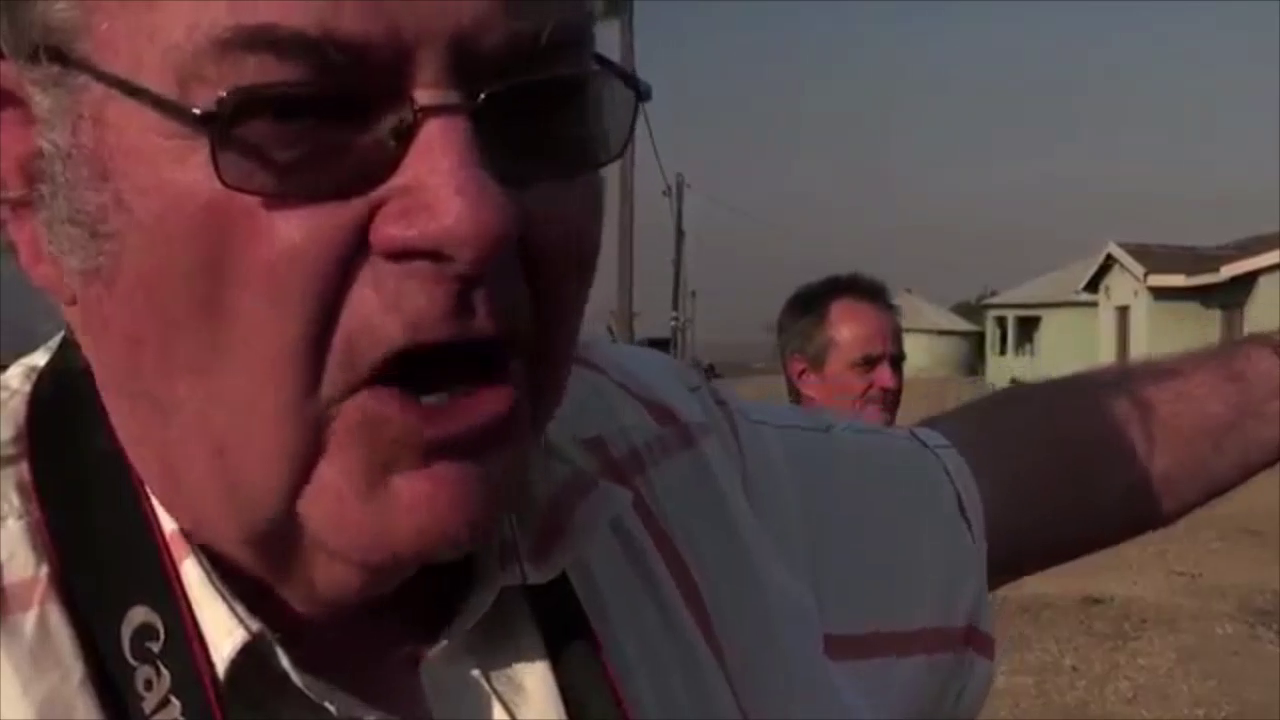
\includegraphics{Figures/play2.png}}{VPlayer.swf}

\end{center}
\end{footnotesize}


\begin{footnotesize}
\texttt{Where our [concern lies is with respect to \annotate{dust}!- because there's no analysis of the dust(.) in terms of the toxic components in that dust]\textsuperscript{1} given the coal mining and the blasting and that sort of thing\degree. Now, you can feel [\annotate{this wind}. <This wind>]\textsuperscript{2} (.) is blowing across us [right into the game reserve]\textsuperscript{3}, so [if] they mine here, this south-easterly wind will carry the dust and the fallout will be in the park, >in the wilderness area<.}   
\end{footnotesize}

\begin{footnotesize}
\begin{enumerate}
   \item Hand in front facing inwards palms open thumbs up
   \item Hands pointing left hand to left
   \item Hand (right) pointing to the right
\end{enumerate}
\end{footnotesize}

\begin{figure}[H]
\centering
\begin{tabular}{llll}

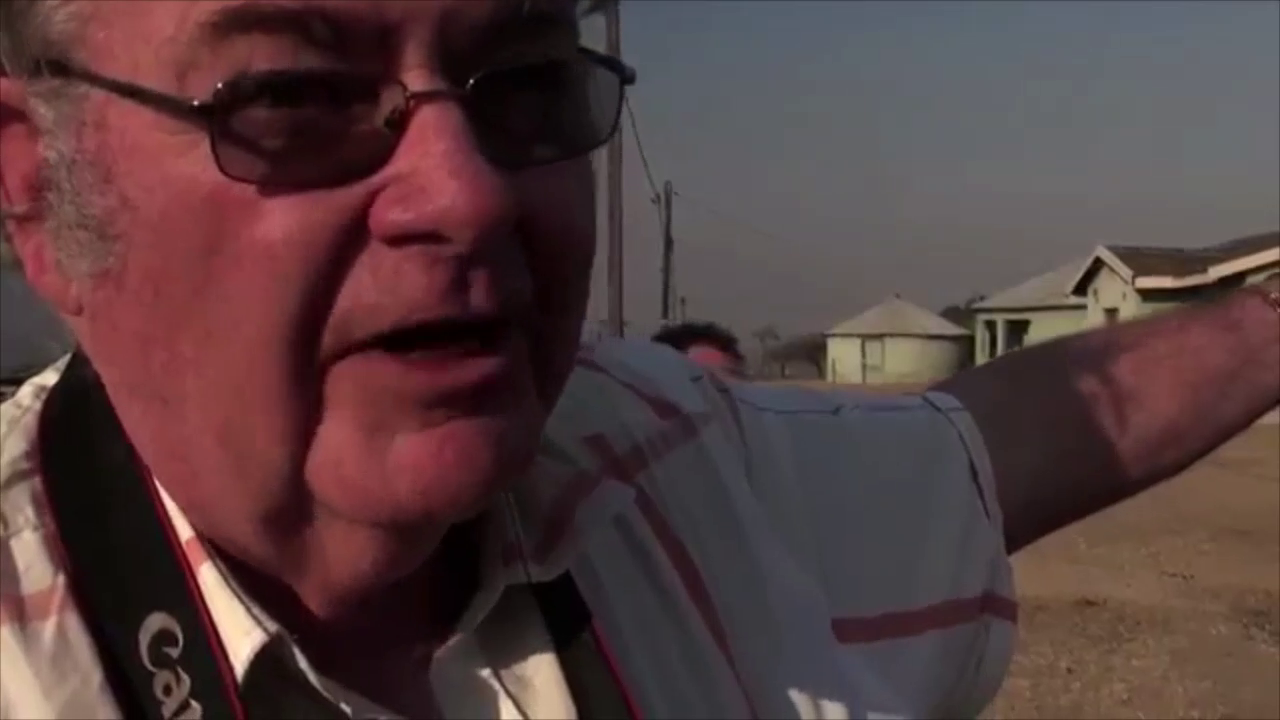
\includegraphics[width=4.2cm]{Figures/mmEco1/frame578.png} & 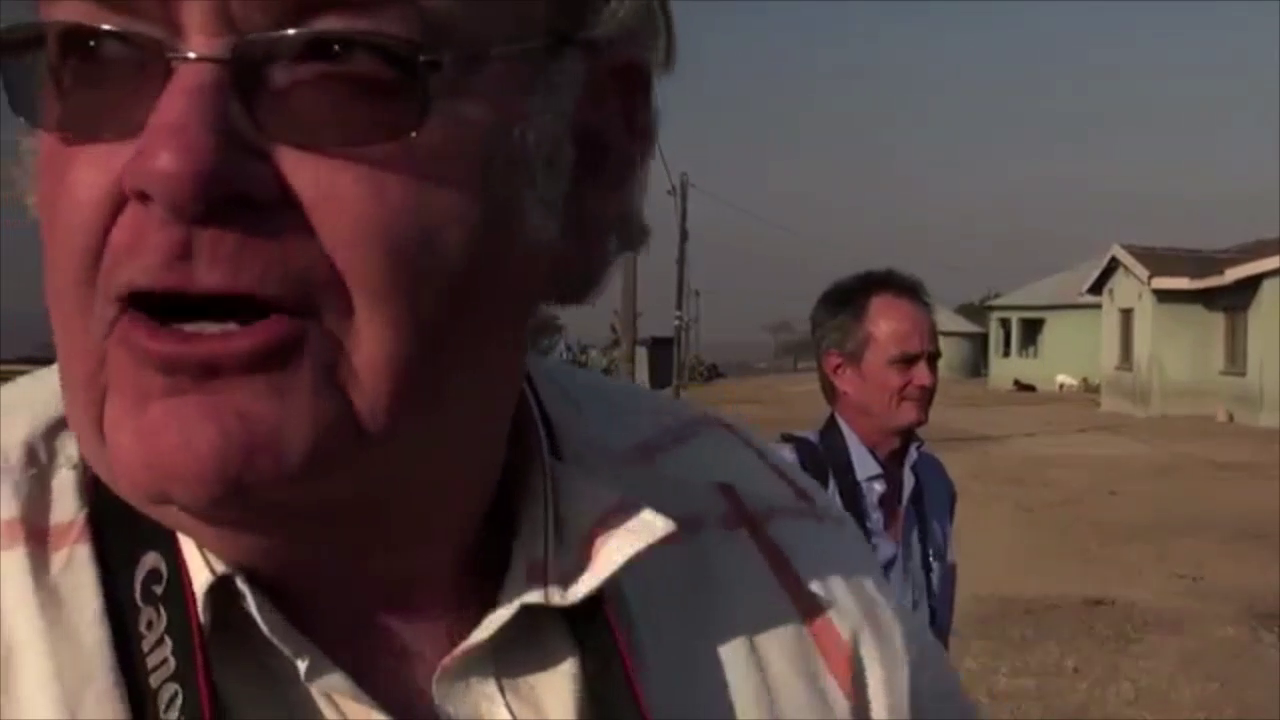
\includegraphics[width=4.2cm]{Figures/mmEco1/frame619.png} & 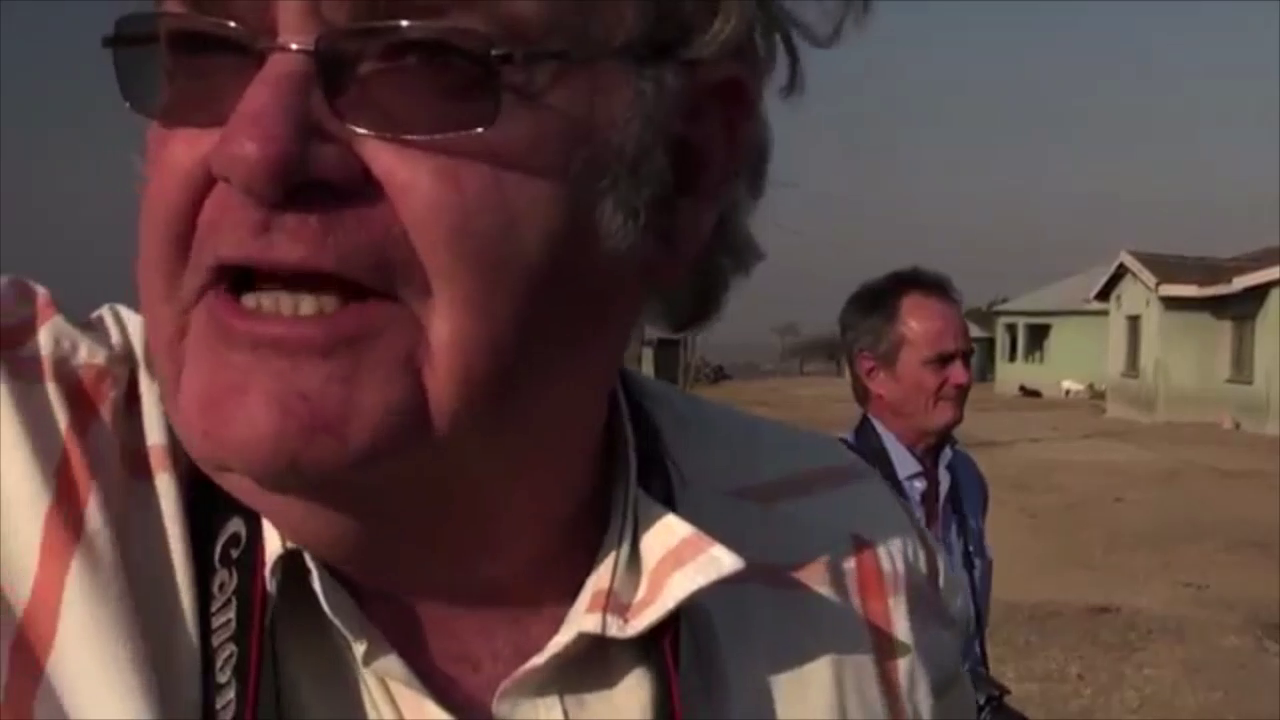
\includegraphics[width=4.2cm]{Figures/mmEco1/frame634.png}  

\end{tabular}
\caption{Ecological Level - Example 2}
\begin{footnotesize}
Hand and arm points to left (Left image) and then to right (Right image) to reflect the physical movement of dust.\\


\end{footnotesize}
\label{fig:figure1}
\end{figure}



\subsection{Ecological Level - Example 3}

\begin{footnotesize}

Source: \url{https://www.youtube.com/embed/UvKe2LYy5pk?start=920&end=945}\\
\textit{Embeded videos require Adobe Flash.}
\begin{center}
\includemedia[width=9.60cm,height=5.40cm,activate=pageopen,
passcontext,
transparent,
addresource=Figures/12.mp4,
flashvars={source=Figures/12.mp4}
]{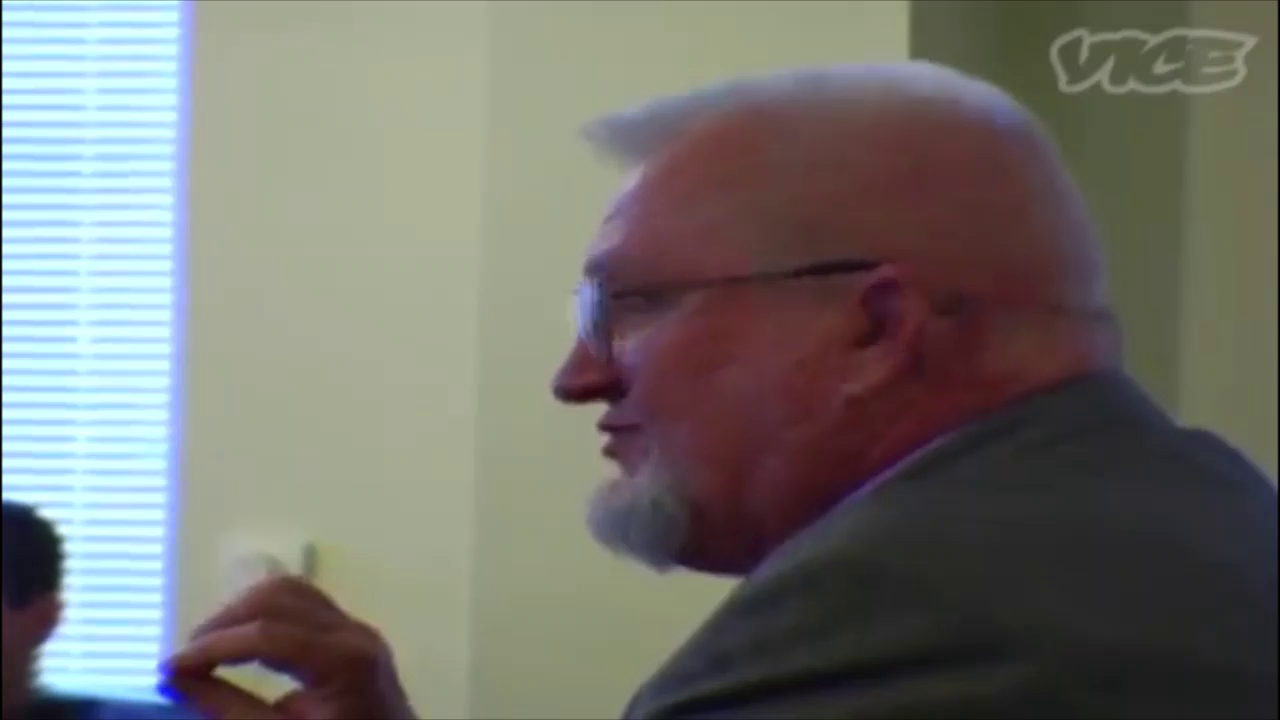
\includegraphics{Figures/play3.png}}{VPlayer.swf}
\end{center}


\begin{footnotesize}
\texttt{People don't understand that <you have to> >[maintain a well just like you do your \annotate{car}]<.\textsuperscript{1} A lot of people just [turn on the spigot,]\textsuperscript{2} and they think [it's going to work for them]\textsuperscript{3} (.) when they have <things like iron hydroxide precipitate> (.) and other metals built up in [their wells (and) every time I go out on a well complaint, I tell people]\textsuperscript{4} you [need to have a friend at the local (.) volunteer fire department come out and flush your well (out)]\textsuperscript{5}....}  
\end{footnotesize}

\begin{footnotesize}
\begin{enumerate}
   \item Index finger and thumb together in precision
   \item Turning of index finger and thumb 
   \item Hand out palm up 
   \item Hand out palm up 
   \item Nodding
\end{enumerate}
\end{footnotesize}

\begin{figure}[H]
\centering
\begin{tabular}{llll}

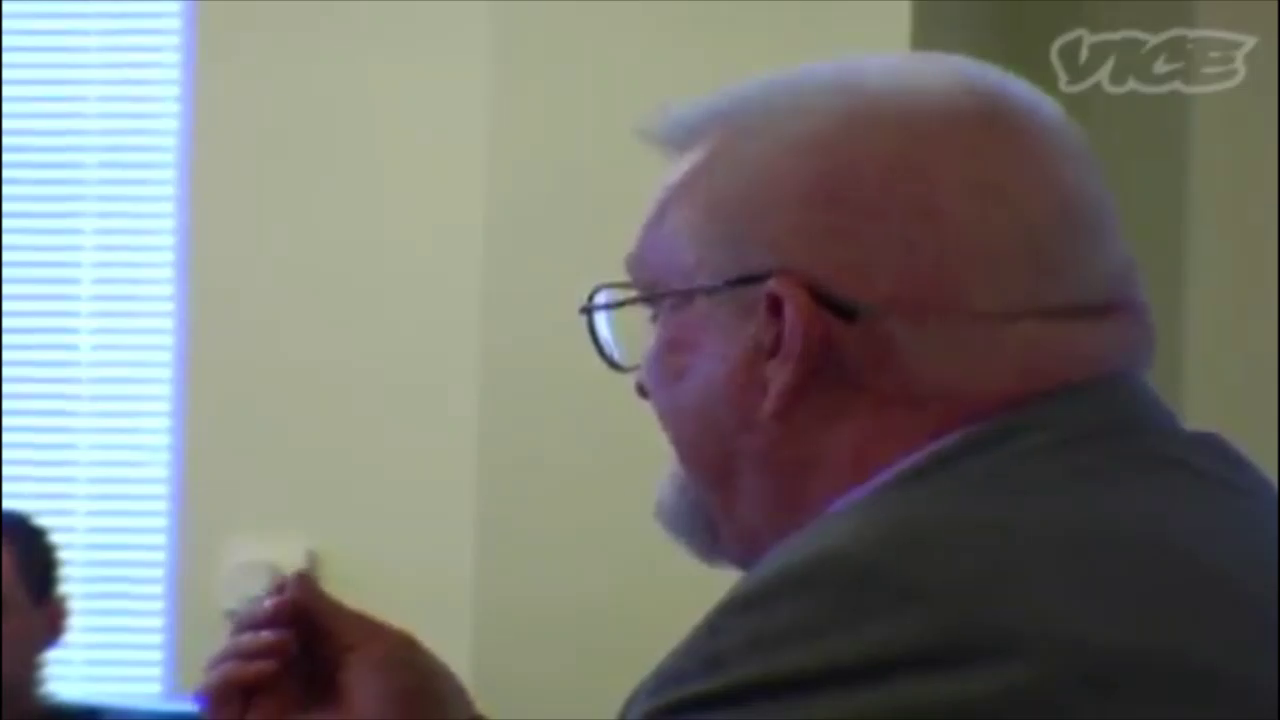
\includegraphics[width=4.2cm]{Figures/mmEco2/frame182.png} & 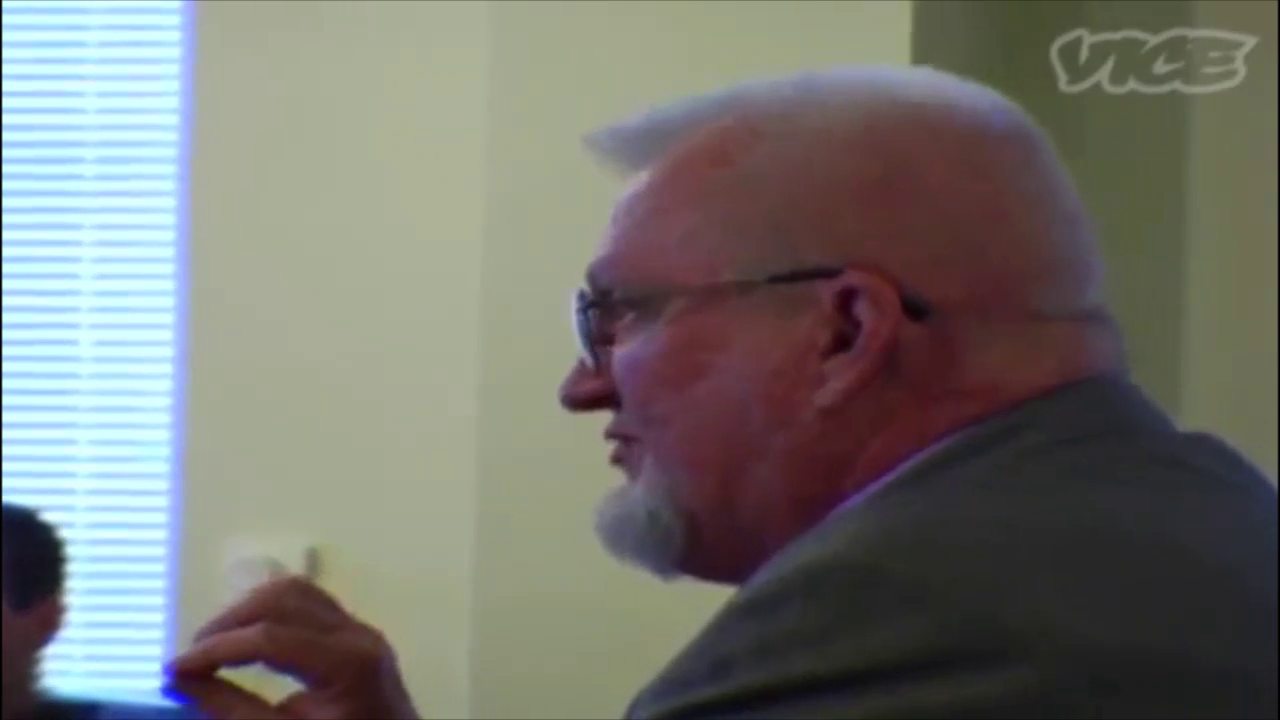
\includegraphics[width=4.2cm]{Figures/mmEco2/frame207.png} & 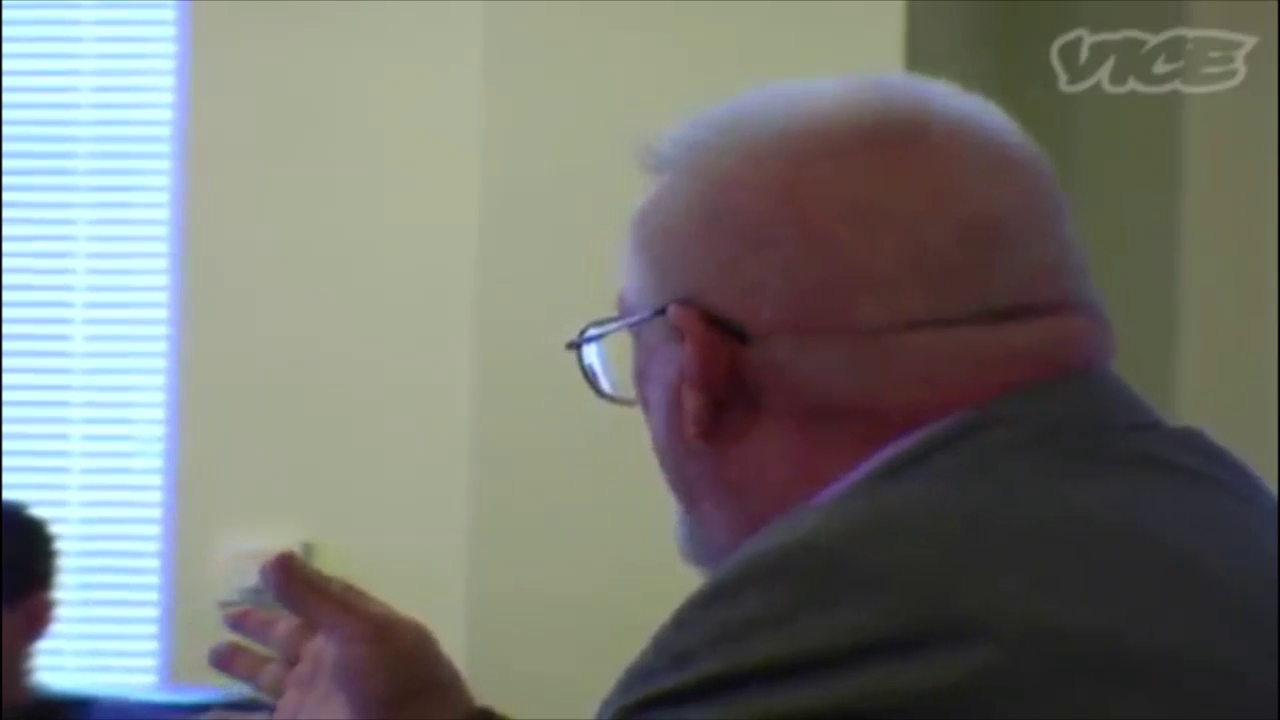
\includegraphics[width=4.2cm]{Figures/mmEco2/frame286.png}  

\end{tabular}
\caption{Ecological Level - Example 3}
\begin{footnotesize}
Left and Middle: the index finger and thumb join to create a precision movement. Right: the open hand palm up gesture functions as a suppliant offer of an idea.\\

\end{footnotesize}
\label{fig:figure1}
\end{figure}

\subsection{Ecological Level - Example 4}

\begin{footnotesize}
Source: \url{https://www.youtube.com/embed/vBhvFWRLiOs?start=821&end=829}\\
\textit{Embeded videos require Adobe Flash.}
\begin{center}
\includemedia[width=9.60cm,height=5.40cm,activate=pageopen,
passcontext,
transparent,
addresource=Figures/18.mp4,
flashvars={source=Figures/18.mp4}
]{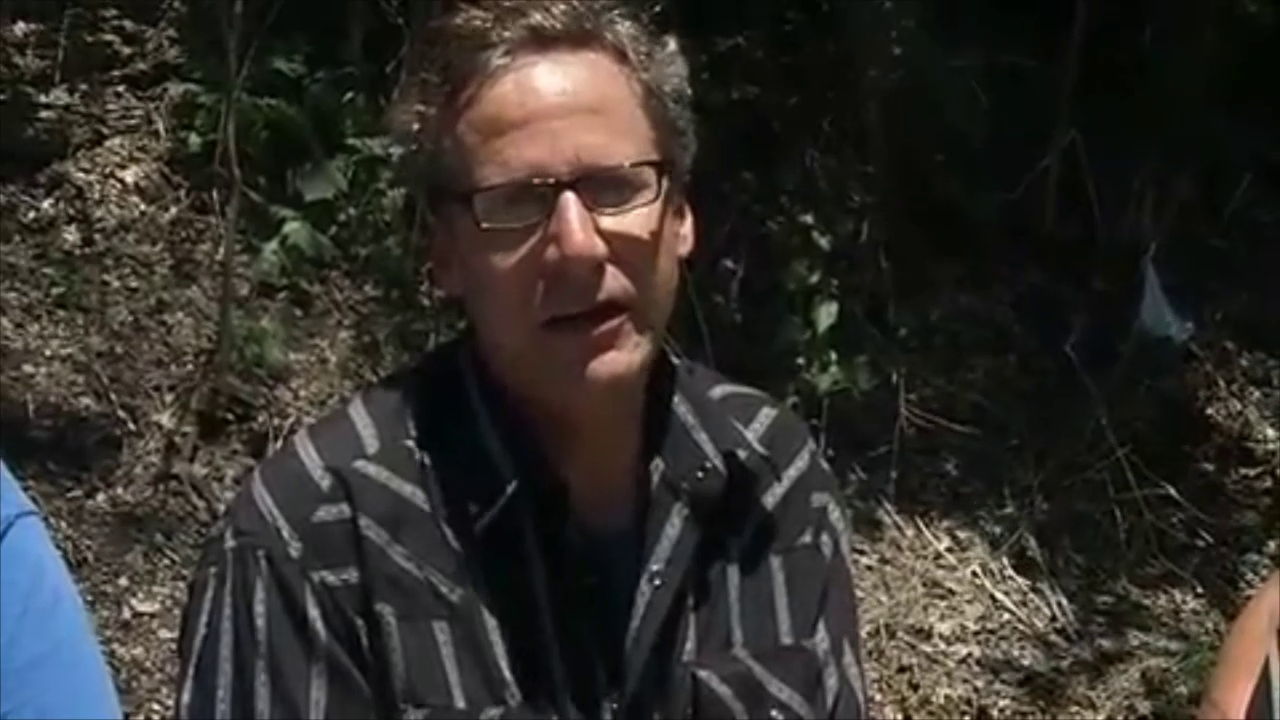
\includegraphics{Figures/play4.png}}{VPlayer.swf}
\end{center}
\end{footnotesize}

\begin{footnotesize}
\texttt{[We've got to build a whole new energy infrastructure for this country, and if we don't we're going to have (.) climate chaos and our kids are going to \annotate{not} thank us for that].\textsuperscript{1}}
\end{footnotesize}

\begin{footnotesize}
\begin{enumerate}
   \item Continuous shaking of HEAD
\end{enumerate}
\end{footnotesize}

\begin{figure}[H]
\centering
\begin{tabular}{llll}

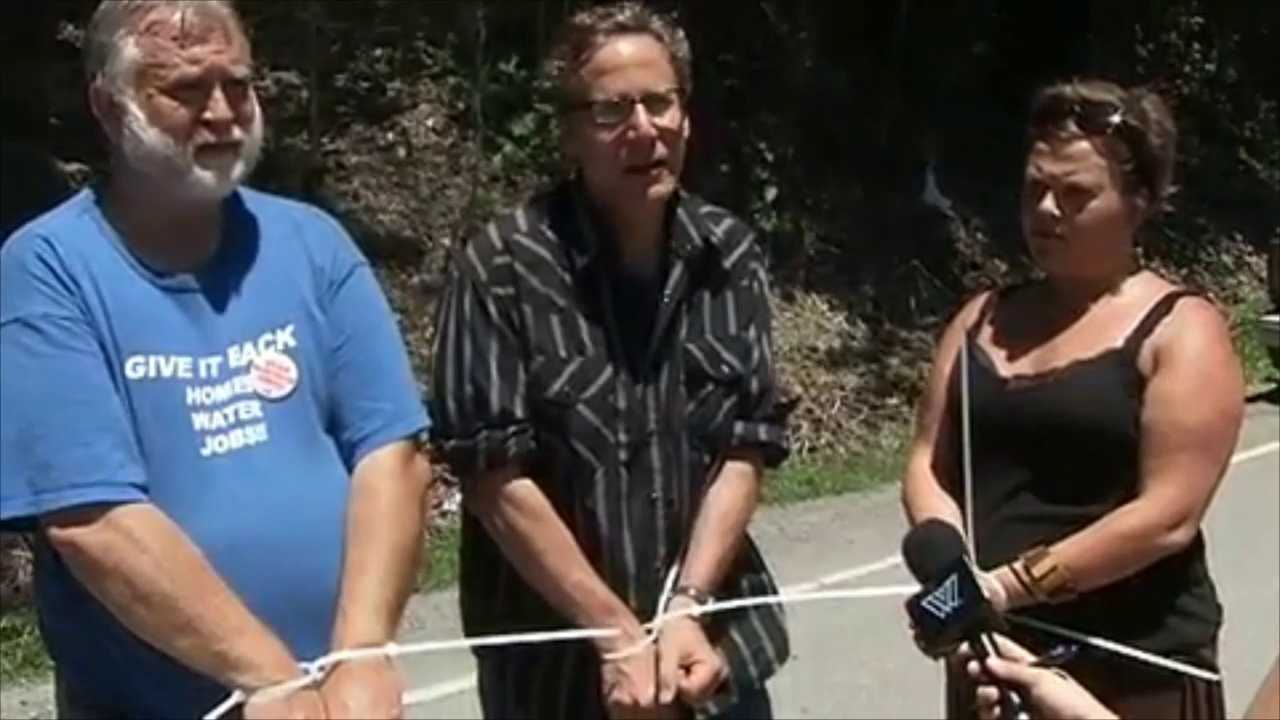
\includegraphics[width=4.2cm]{Figures/mmEco4/frame8.png} & 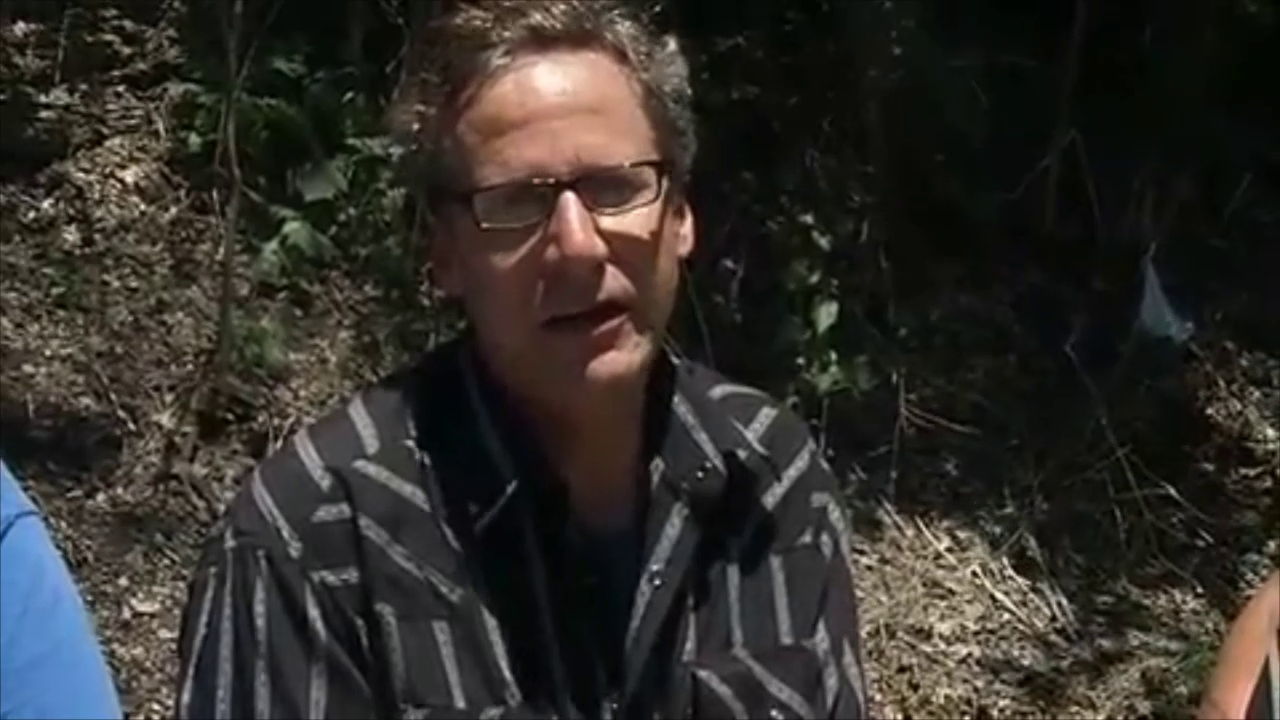
\includegraphics[width=4.2cm]{Figures/mmEco4/frame192.png} & 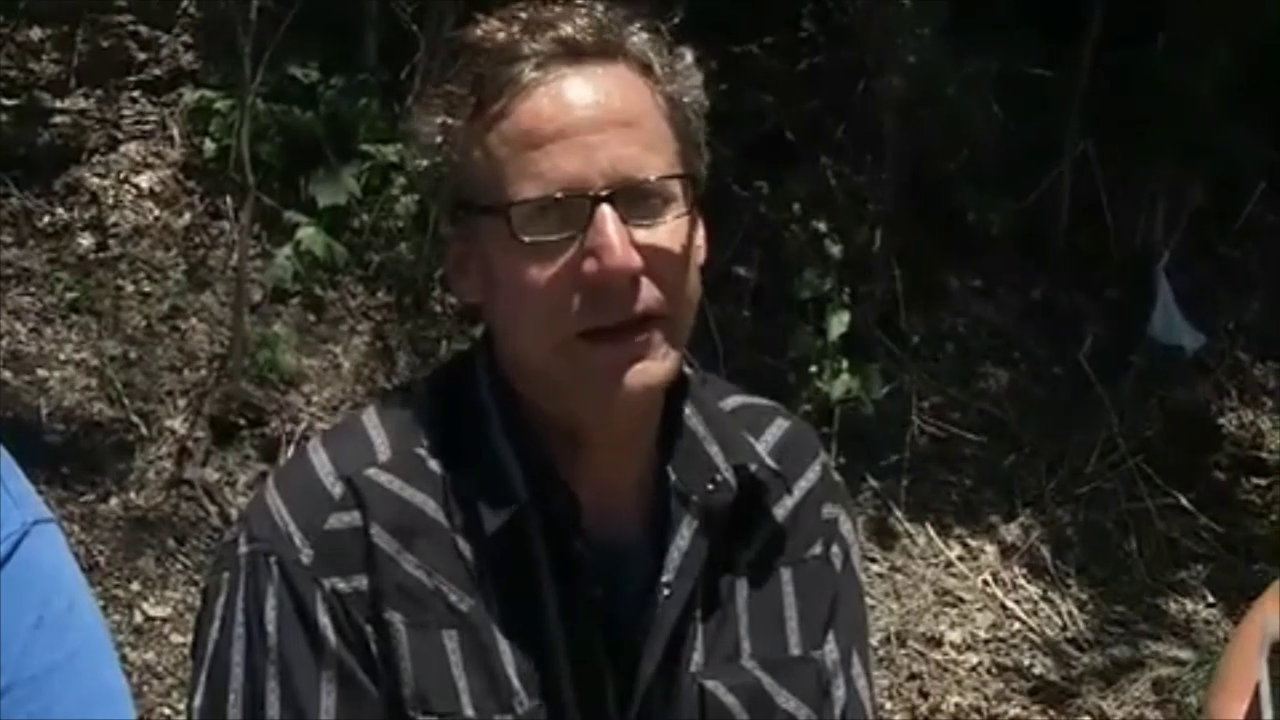
\includegraphics[width=4.2cm]{Figures/mmEco4/frame219.png}  

\end{tabular}
\caption{Ecological Level - Example 4}

\begin{footnotesize}
Left: hands constrained, possible accentuating communicative head movements. Middle, Right: continuous movement (shaking) of head from left to right carrying the meaning of unbelievable.\\

\end{footnotesize}
\label{fig:figure1}
\end{figure}


\section{Cultural-Level}

\subsection{Cultural Level - Example 1}

\begin{footnotesize}
Source: \url{https://www.youtube.com/embed/z6ewpjWYfYo?start=535&end=555}\\
\textit{Embeded videos require Adobe Flash.}
\begin{center}
\includemedia[width=9.60cm,height=5.40cm,activate=pageopen,
passcontext,
transparent,
addresource=Figures/02.mp4,
flashvars={source=Figures/02.mp4}
]{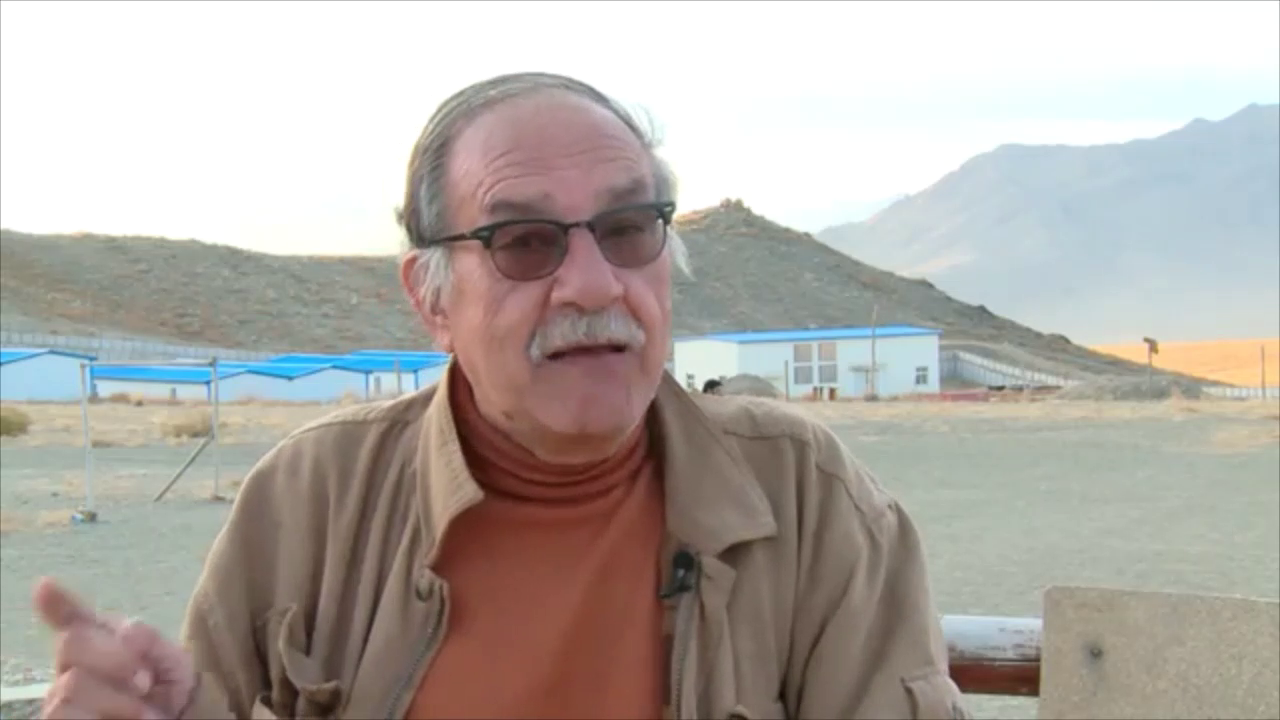
\includegraphics{Figures/play5.png}}{VPlayer.swf}
\end{center}
\end{footnotesize}


\begin{footnotesize}
\texttt{...with [all these wars (over) 30, 40 years]\textsuperscript{1}, (.) what the Afghan has lost we lost [our identity]\textsuperscript{2}!- and [I \annotate{believe}]\textsuperscript{3} to give (them) \annotate{back} that identity is only through [\annotate{culture}]\textsuperscript{4} !- because when it [\annotate{comes}]\textsuperscript{5} to culture, all Afghans are united.}
\end{footnotesize}

\begin{footnotesize}
\begin{enumerate}
   \item Left hand forward palm up; lateral sweep of head and hand
   \item Right hand motion to side; index finger extended; eyebrows raise
   \item Right hand motion to side; index finger extended; head tilts to one side
   \item Right hand motion forward; index finger extended
   \item Right hand motion forward; index finger extended; intonation on ``comes''
\end{enumerate}
\end{footnotesize}

\begin{figure}[H]
\centering
\begin{tabular}{llll}
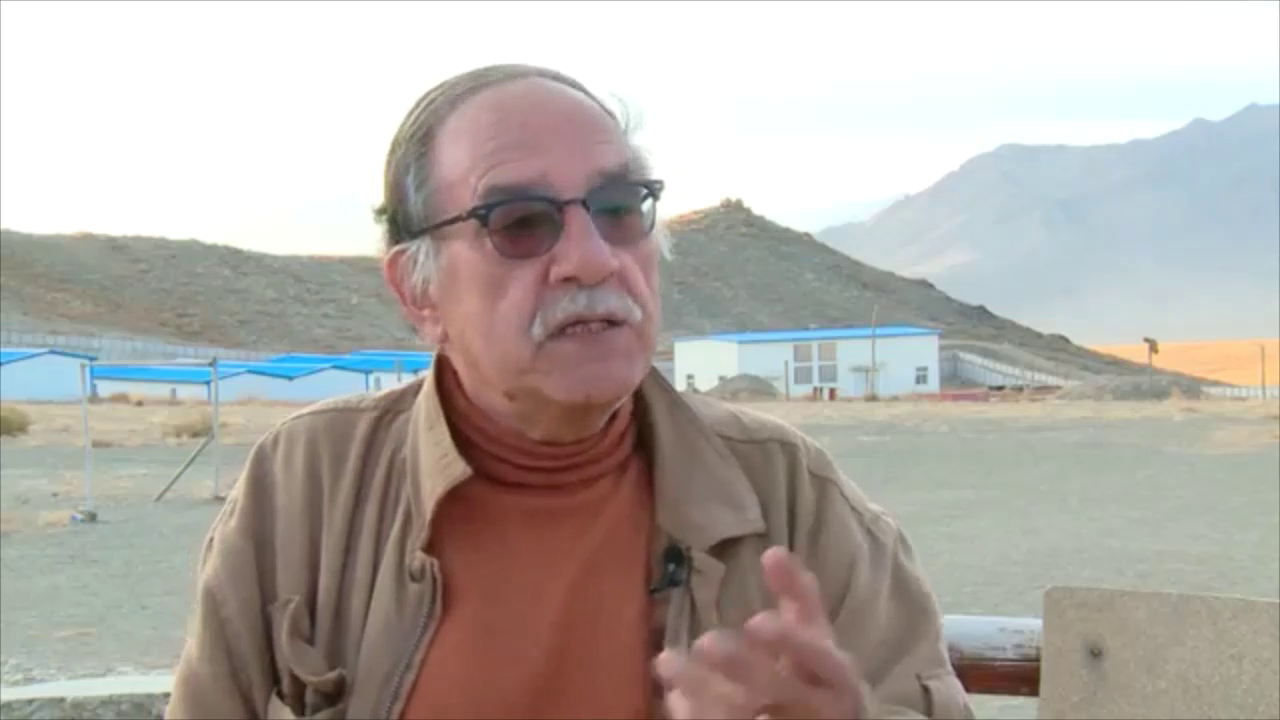
\includegraphics[width=4.2cm]{Figures/mmCult1/frame15.png} & 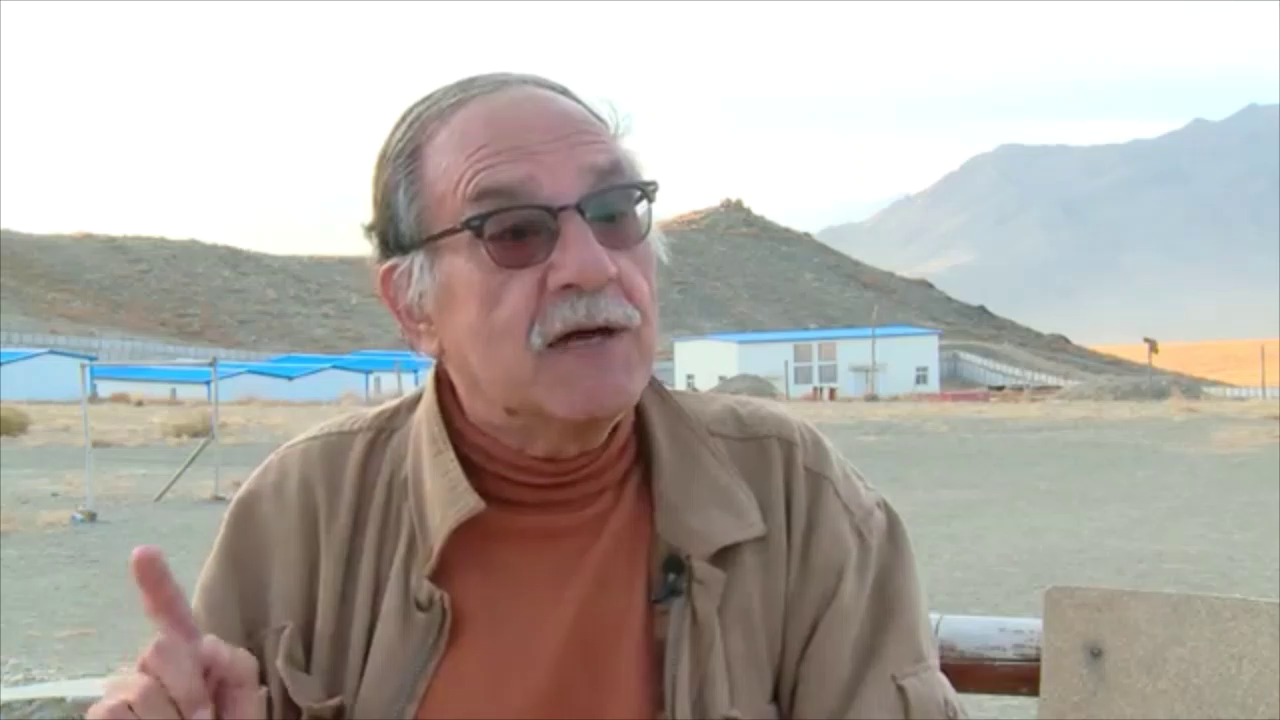
\includegraphics[width=4.2cm]{Figures/mmCult1/frame241.png} & 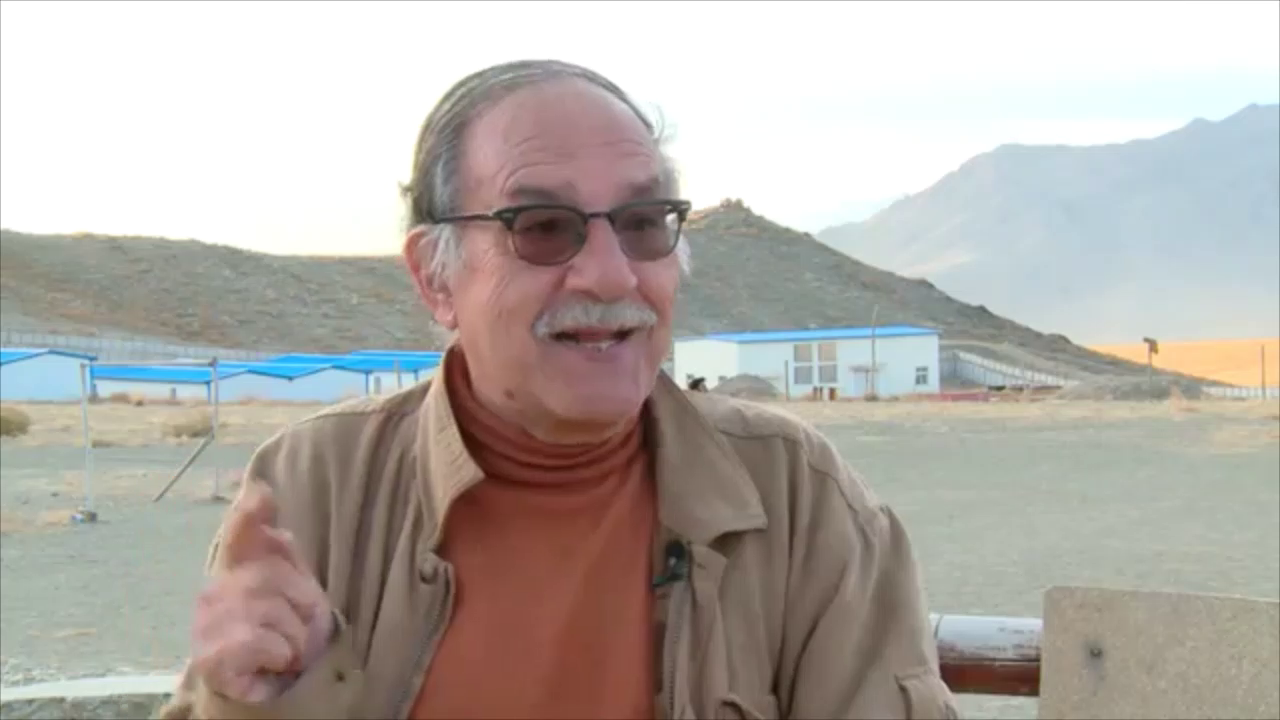
\includegraphics[width=4.2cm]{Figures/mmCult1/frame513.png} 

\end{tabular}
\caption{Cultural level - Example 1}
\begin{footnotesize}

\end{footnotesize}
\label{fig:figure1}
\end{figure}




\subsection{Cultural Level - Example 2}

\begin{footnotesize}
Source: \url{https://www.youtube.com/embed/10FrfEa0Xck?start=33&end=45}\\
\textit{Embeded videos require Adobe Flash.}
\begin{center}
\includemedia[width=9.60cm,height=5.40cm,activate=pageopen,
passcontext,
transparent,
addresource=Figures/03.mp4,
flashvars={source=Figures/03.mp4}
]{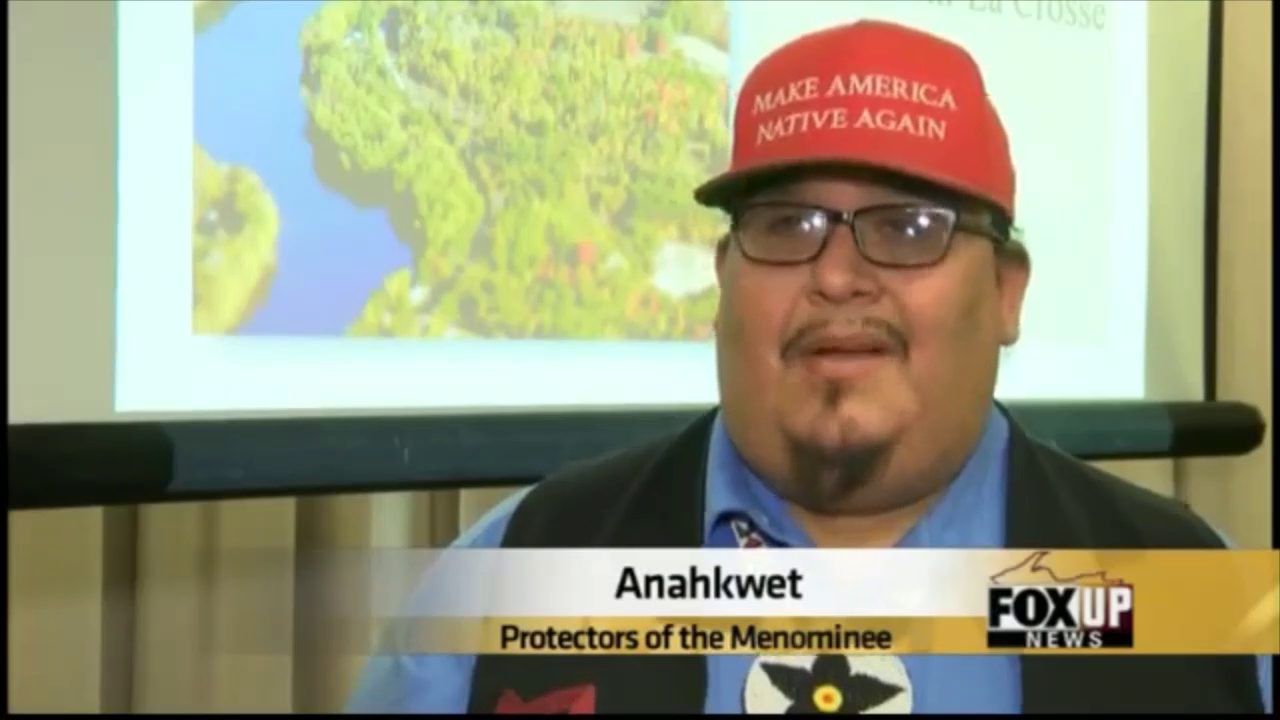
\includegraphics{Figures/mmCult2/frame202.png}}{VPlayer.swf}
\end{center}
\end{footnotesize}




\begin{footnotesize}
\texttt{(It's) [my prehistoric ancestors] (.) that are right within this mining area and [I don't want (.) .hhh hhh you know]\textsuperscript{2} [any \annotate{mine}]\textsuperscript{3} near them, >I don't want any equipment near them.< We have <three known \annotate{burial}> (mound) groups that are there.} 
\end{footnotesize}

\begin{footnotesize}
\begin{enumerate}
   \item Nodding head on beat
   \item Shaking head
   \item Left lip tightened and raised; slight raising of shoulders
\end{enumerate}
\end{footnotesize}

\begin{figure}[H]
\centering
\begin{tabular}{llll}
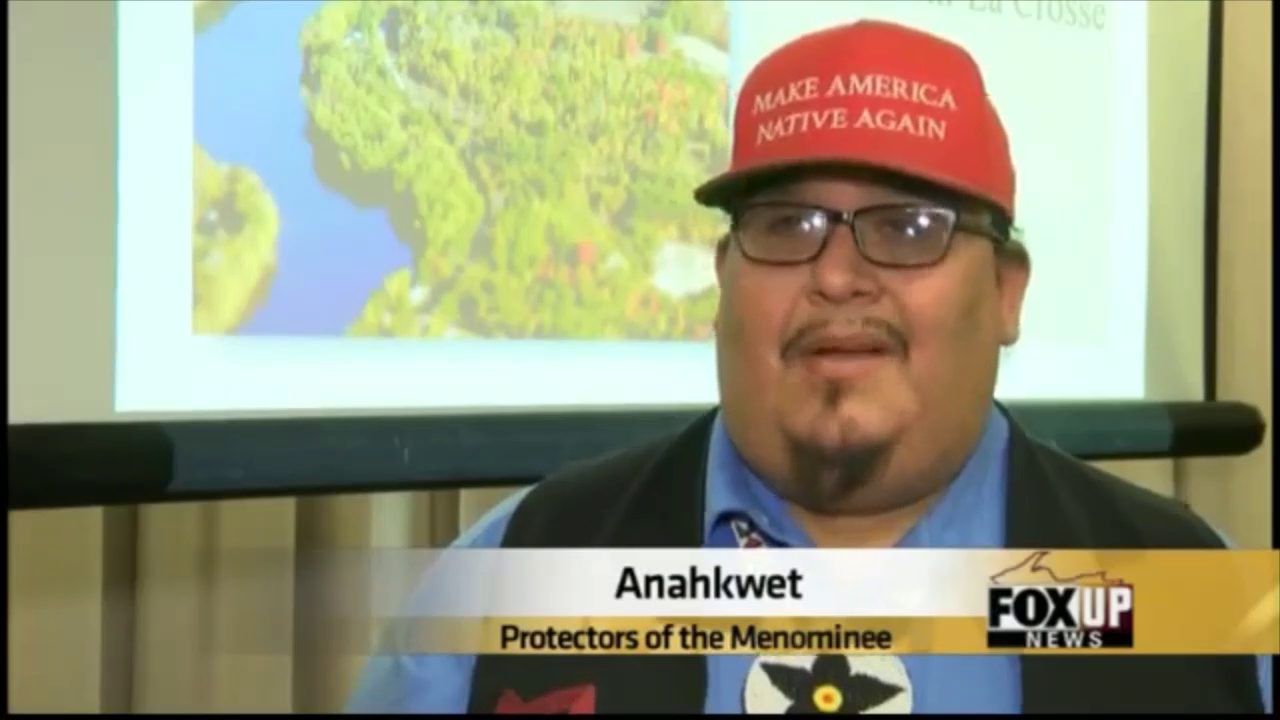
\includegraphics[width=4.2cm]{Figures/mmCult2/frame202.png} & 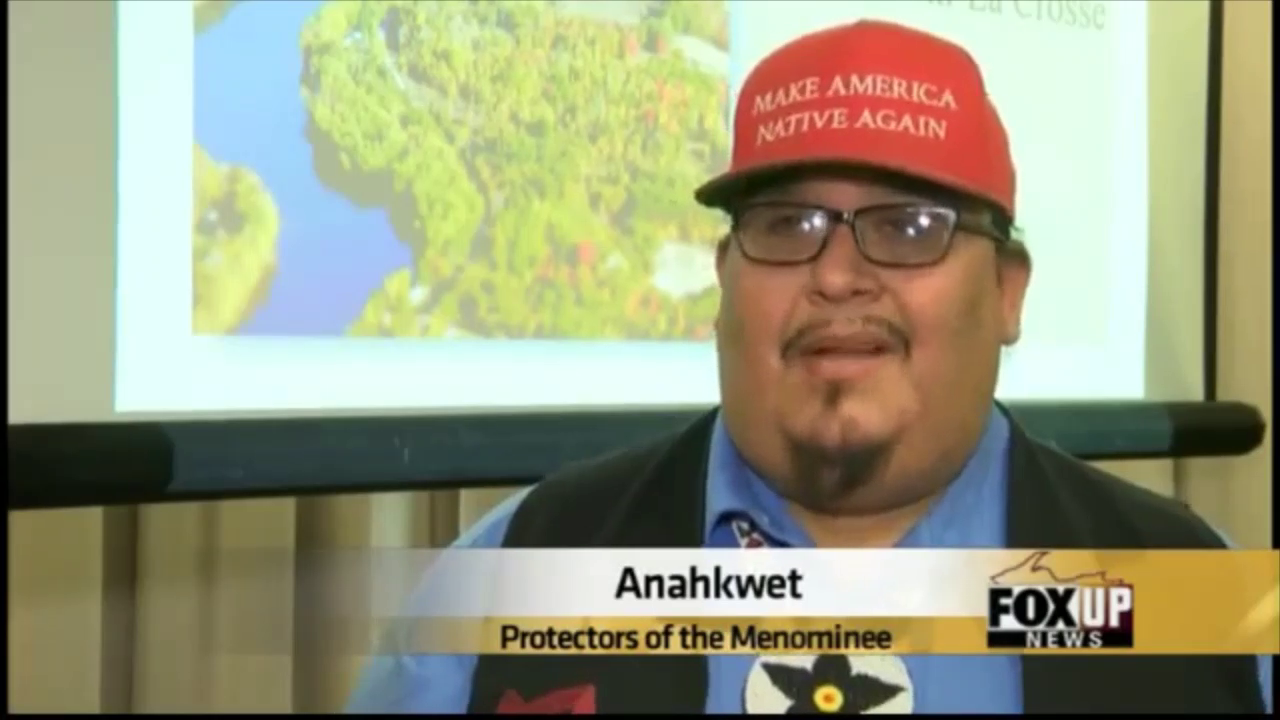
\includegraphics[width=4.2cm]{Figures/mmCult2/frame203.png} & 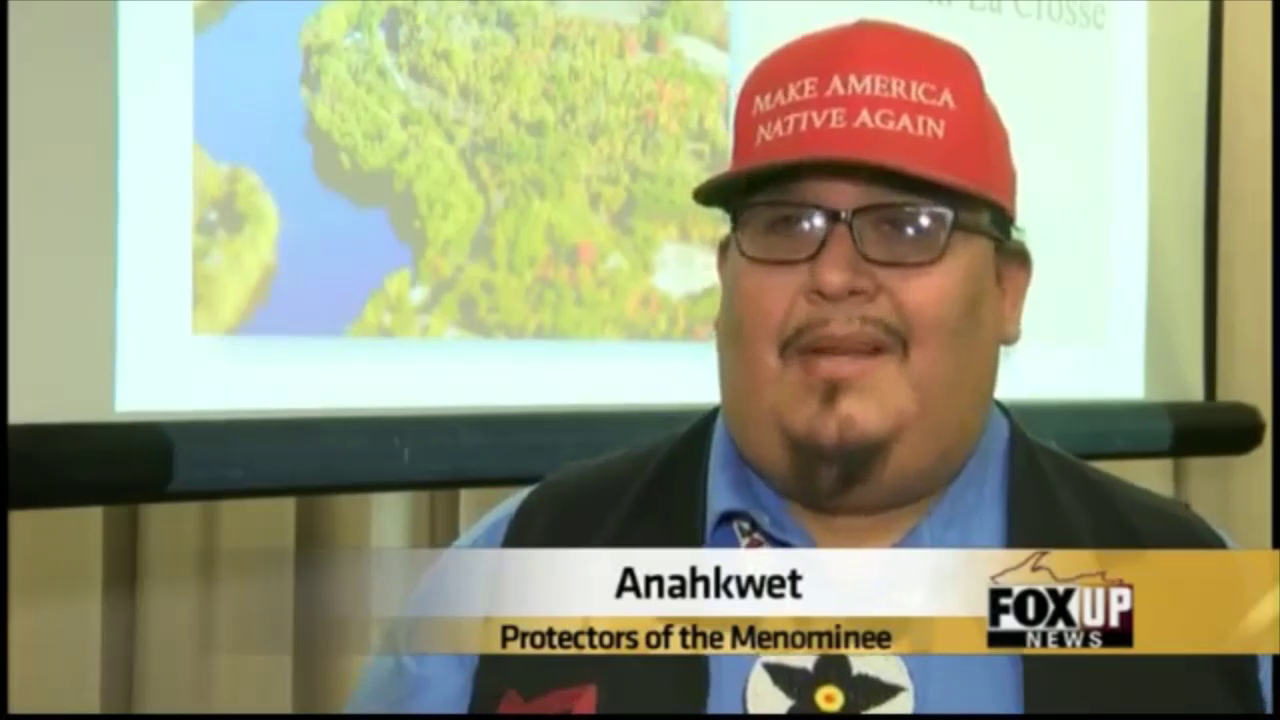
\includegraphics[width=4.2cm]{Figures/mmCult2/frame204.png} 

\end{tabular}
\caption{Cultural level - Example 2}
\begin{footnotesize}

\end{footnotesize}
\label{fig:figure1}
\end{figure}


\subsection{Cultural Level - Example 3}

\begin{footnotesize}
Source: \url{https://www.youtube.com/embed/awnLI4pRnUM?start=42&end=58}\\
\textit{Embeded videos require Adobe Flash.}
\begin{center}
\includemedia[width=9.60cm,height=5.40cm,activate=pageopen,
passcontext,
transparent,
addresource=Figures/04.mp4,
flashvars={source=Figures/04.mp4}
]{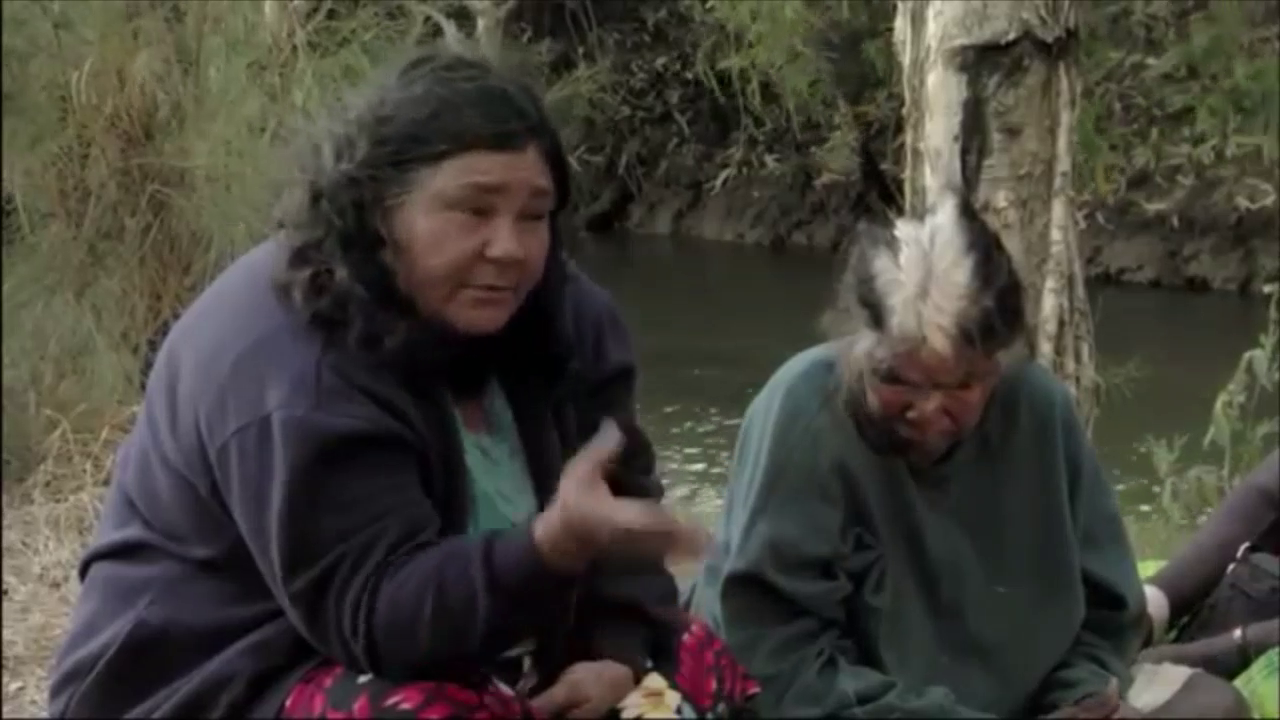
\includegraphics{Figures/mmCult3/frame75.png}}{VPlayer.swf}
\end{center}
\end{footnotesize}



\begin{footnotesize}
\texttt{<[They crushed out sacred site]>. They never [listened to aboriginal people, <elders, female elders>] (.) you know they've been [\annotate{stomped} on]. So it's time for them to \annotate{stand} up and say [hey you're not doing this to me anymore].} 
\end{footnotesize}

\begin{footnotesize}
\begin{enumerate}
   \item Right hand motion forward on beat; palm up; index finger and thumb touching
   \item Right hand motion forward on beat; palm up; fingers and thumb open; high blink rate
   \item Head swipe, left to right with emphasis
   \item Head motion with clenched fist
\end{enumerate}
\end{footnotesize}

\begin{figure}[H]
\centering
\begin{tabular}{llll}

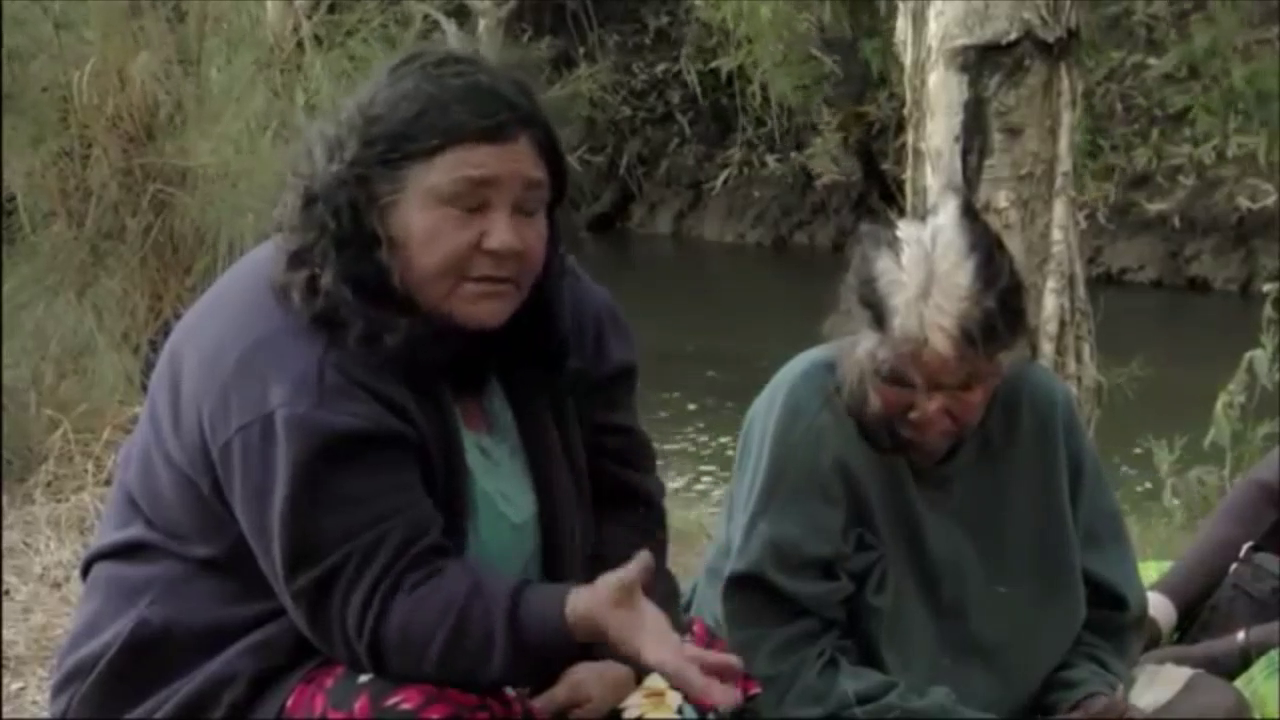
\includegraphics[width=4.2cm]{Figures/mmCult3/frame85.png} & 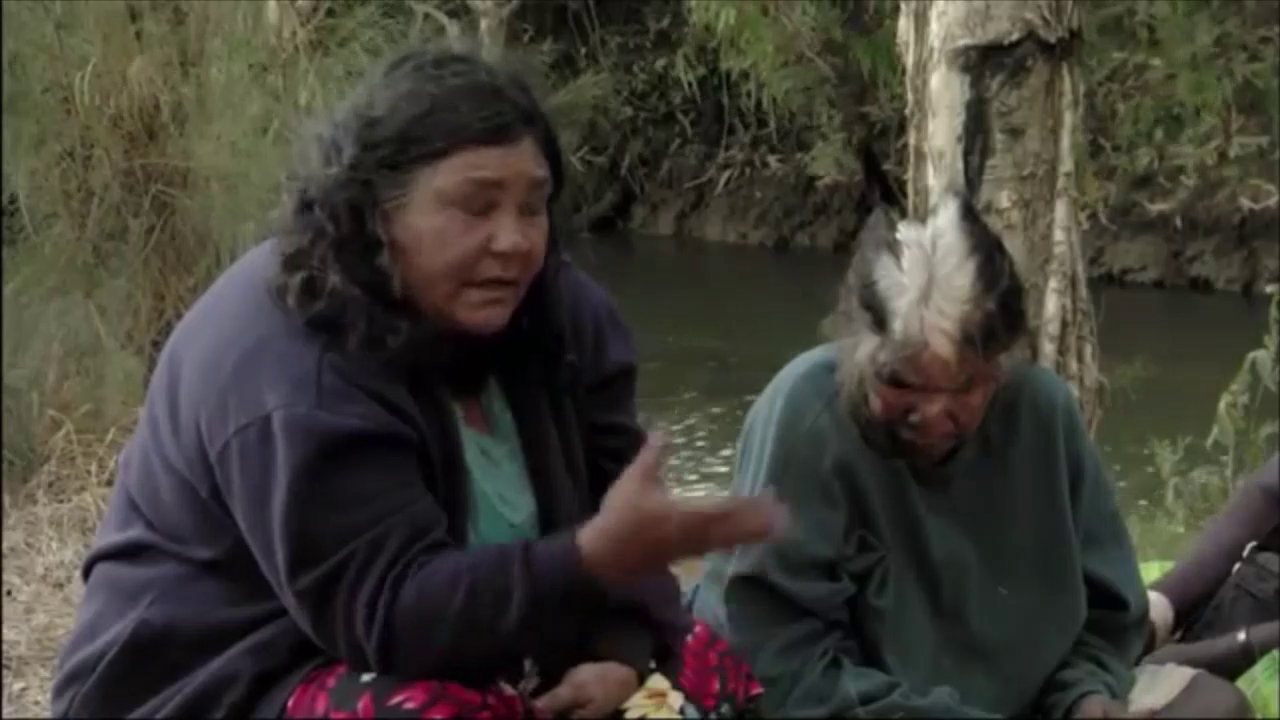
\includegraphics[width=4.2cm]{Figures/mmCult3/frame128.png} & 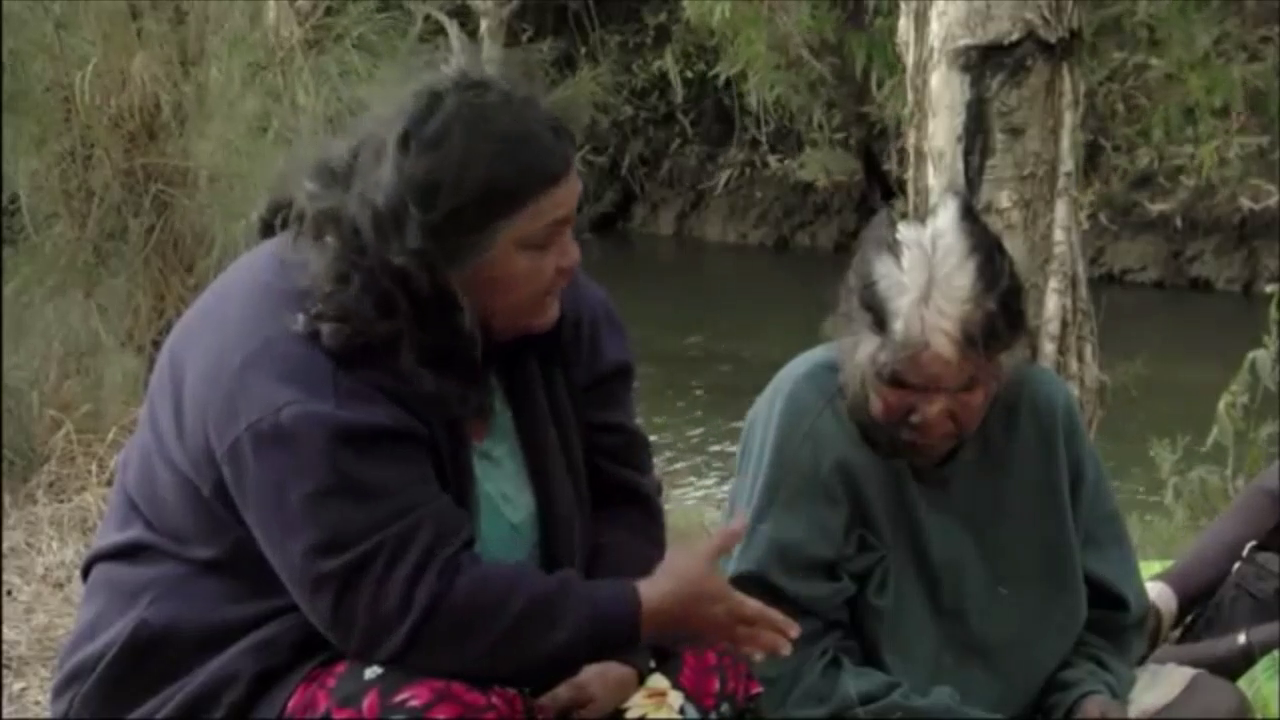
\includegraphics[width=4.2cm]{Figures/mmCult3/frame141.png}  

\end{tabular}
\caption{Cultural Level - Example 3}
\begin{footnotesize}

\end{footnotesize}
\label{fig:figure1}
\end{figure}



\subsection{Cultural Level - Example 4}

\begin{footnotesize}
Source: \url{https://www.youtube.com/embed/UvKe2LYy5pk?start=1198&end=1220}\\\\
\textit{Embeded videos require Adobe Flash.}
\begin{center}
\includemedia[width=9.60cm,height=5.40cm,activate=pageopen,
passcontext,
transparent,
addresource=Figures/14.mp4,
flashvars={source=Figures/14.mp4}
]{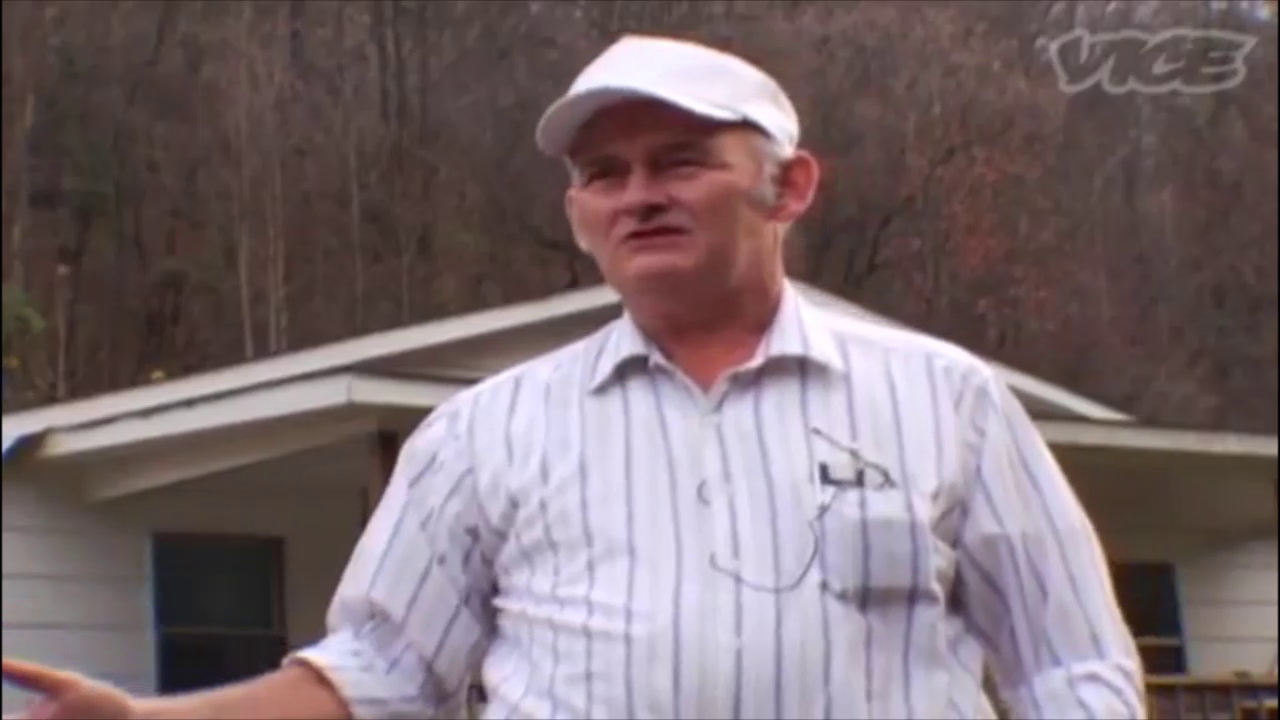
\includegraphics{Figures/mmCult4/frame218.png}}{VPlayer.swf}
\end{center}
\end{footnotesize}


\textbf{\underline{Cultural Level - Example 4}}

\begin{footnotesize}
\texttt{You \annotate{pray} before you go to bed... and >you just ask God to protect (you and) your family, that's all you \annotate{can} do,< because (.) [\annotate{man} has done the damage to the earth (.) and man]\textsuperscript{1} (.) [I don't see how <man can correct what's been done>]\textsuperscript{2}. [\annotate{God} can handle this (.) and he will. When the right time comes]\textsuperscript{3}, he will do what needs to be done.}
\end{footnotesize}

\begin{footnotesize}
\begin{enumerate}
   \item Right hand motions forward; palm up
   \item Right hand motions forward, fingers and thumbs curled inward; head shaking
   \item Rand waves outwards, stops at thigh; gaze upwards to sky; nodding 
\end{enumerate}
\end{footnotesize}

\begin{figure}[H]
\centering
\begin{tabular}{llll}

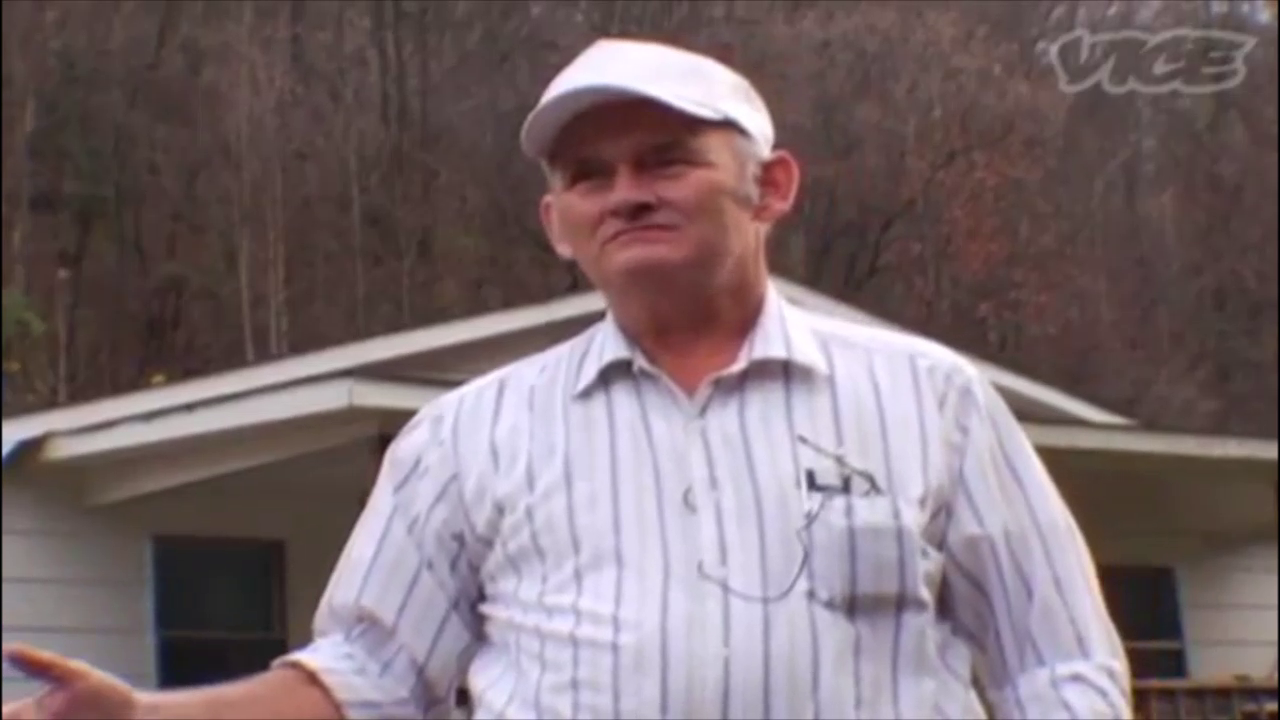
\includegraphics[width=4.2cm]{Figures/mmCult4/frame237.png} & 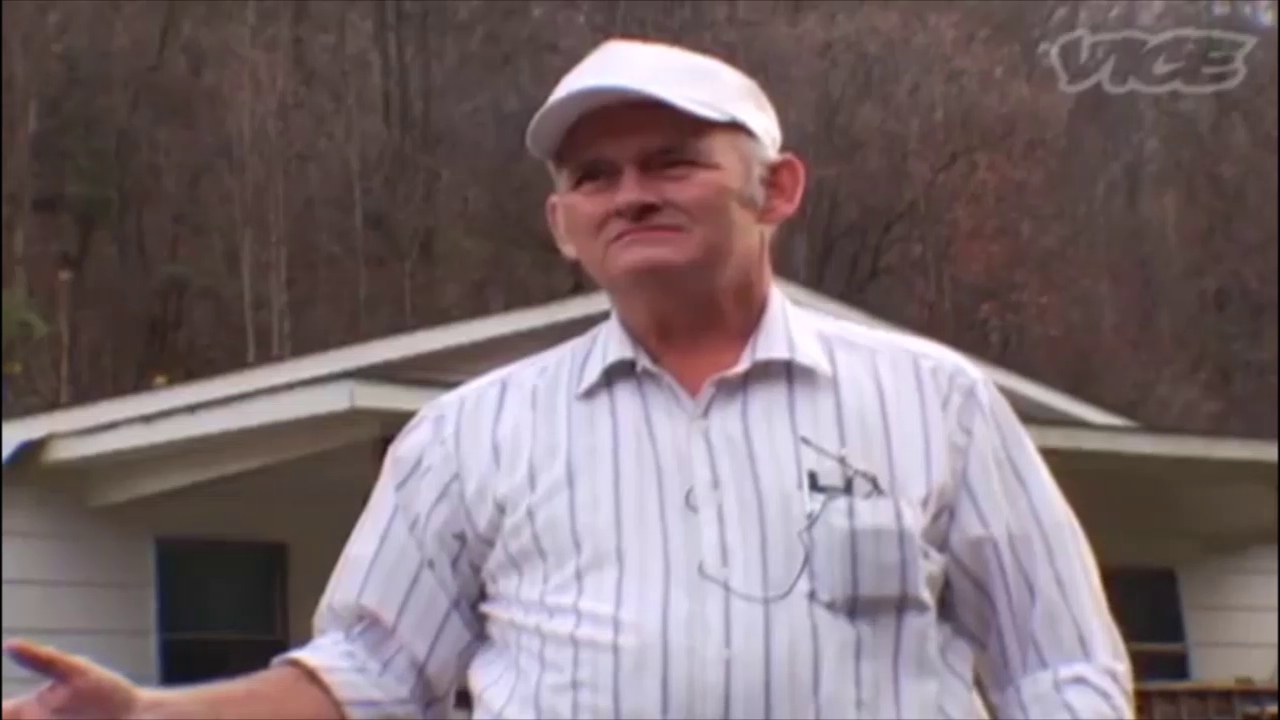
\includegraphics[width=4.2cm]{Figures/mmCult4/frame245.png} & 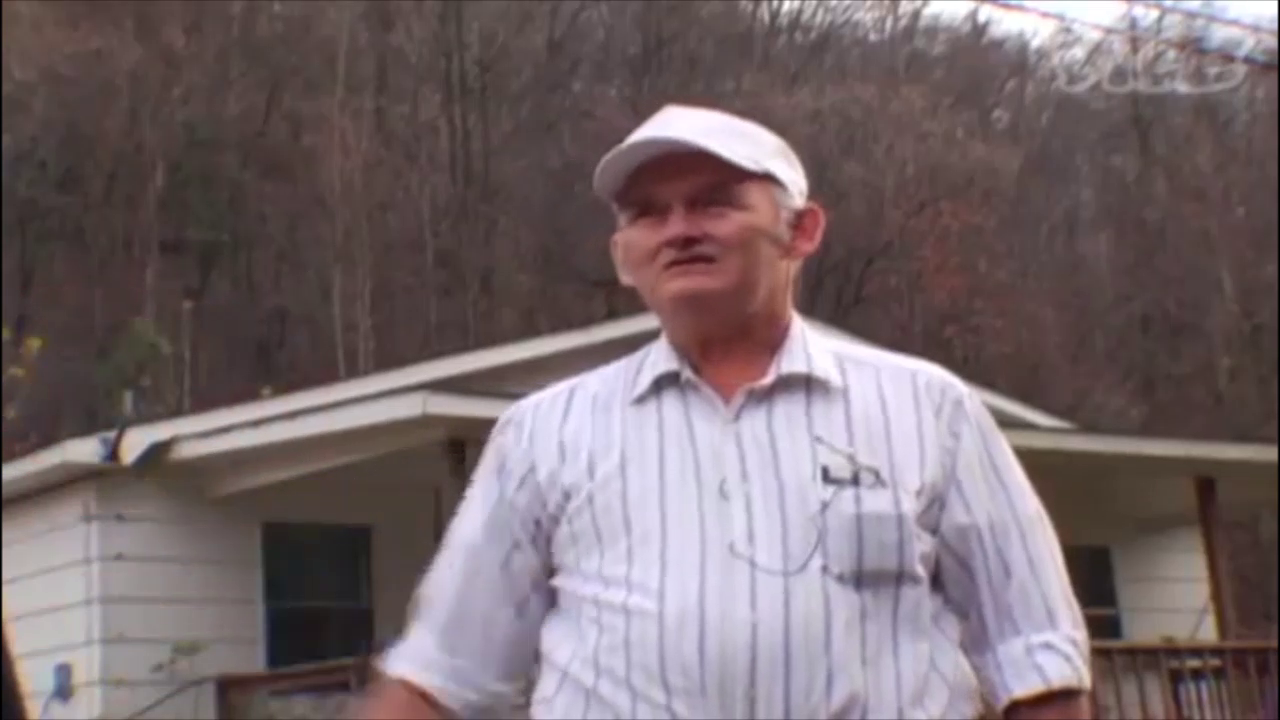
\includegraphics[width=4.2cm]{Figures/mmCult4/frame437.png}  

\end{tabular}
\caption{Cultural level - Example 4}
\begin{footnotesize}

\end{footnotesize}
\label{fig:figure1}
\end{figure}



\subsection{Cultural Level - Example 5}

\begin{footnotesize}
Source: \url{https://www.youtube.com/embed/vBhvFWRLiOs?start=467&end=476}\\
\textit{Embeded videos require Adobe Flash.}
\begin{center}
\includemedia[width=9.60cm,height=5.40cm,activate=pageopen,
passcontext,
transparent,
addresource=Figures/17.mp4,
flashvars={source=Figures/17.mp4}
]{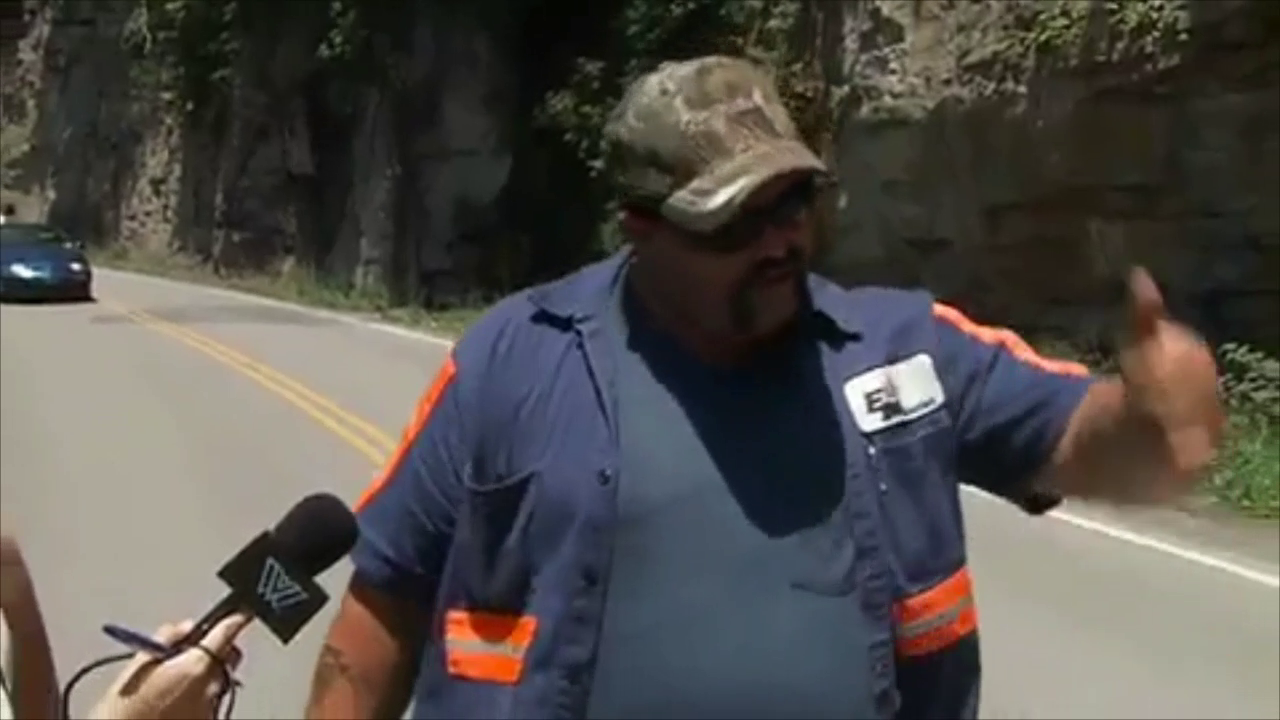
\includegraphics{Figures/mmCult5/frame103.png}}{VPlayer.swf}
\end{center}
\end{footnotesize}

\begin{footnotesize}
\texttt{If [they're for us]\textsuperscript{1}, that's good. If they're [against us, get out]\textsuperscript{2} of the state.}
\end{footnotesize}

\begin{footnotesize}
\begin{enumerate}
   \item Hand motion down towards ground, index finger extended
   \item Thumb up; hand motion back over left shoulder
\end{enumerate}
\end{footnotesize}

\begin{figure}[H]
\centering
\begin{tabular}{llll}

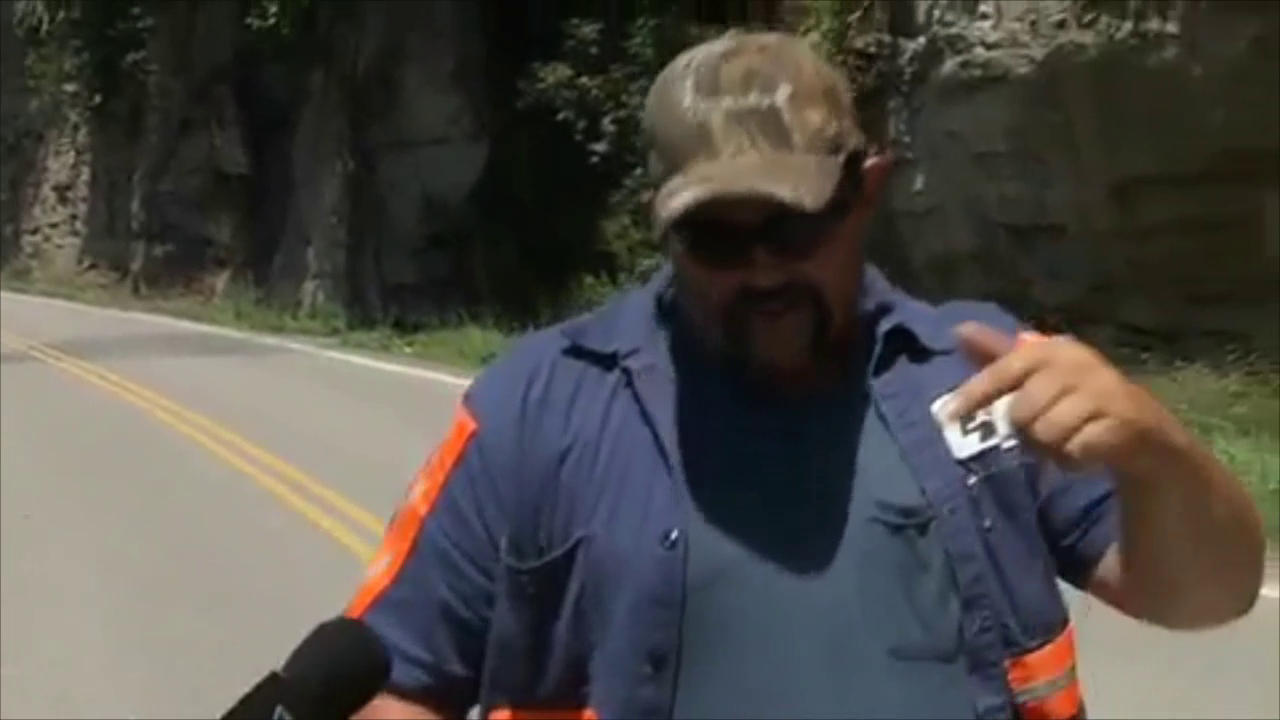
\includegraphics[width=4.2cm]{Figures/mmCult5/frame19.png} & 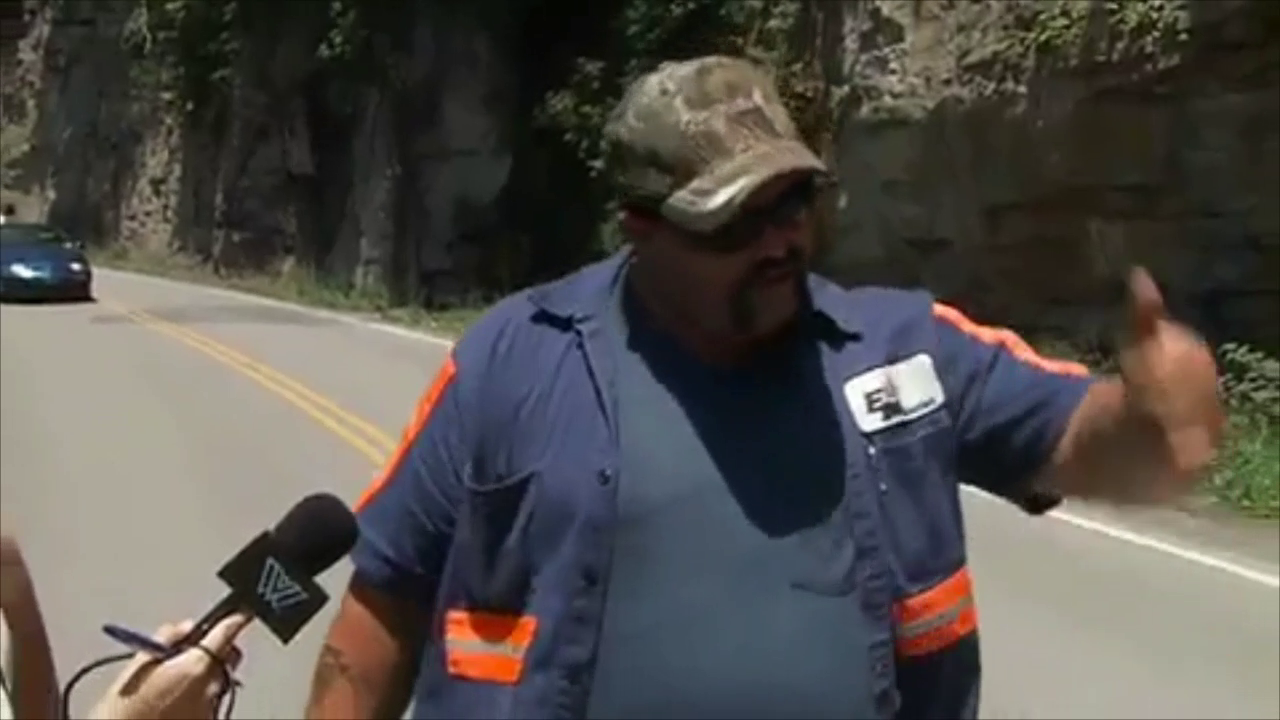
\includegraphics[width=4.2cm]{Figures/mmCult5/frame103.png} & 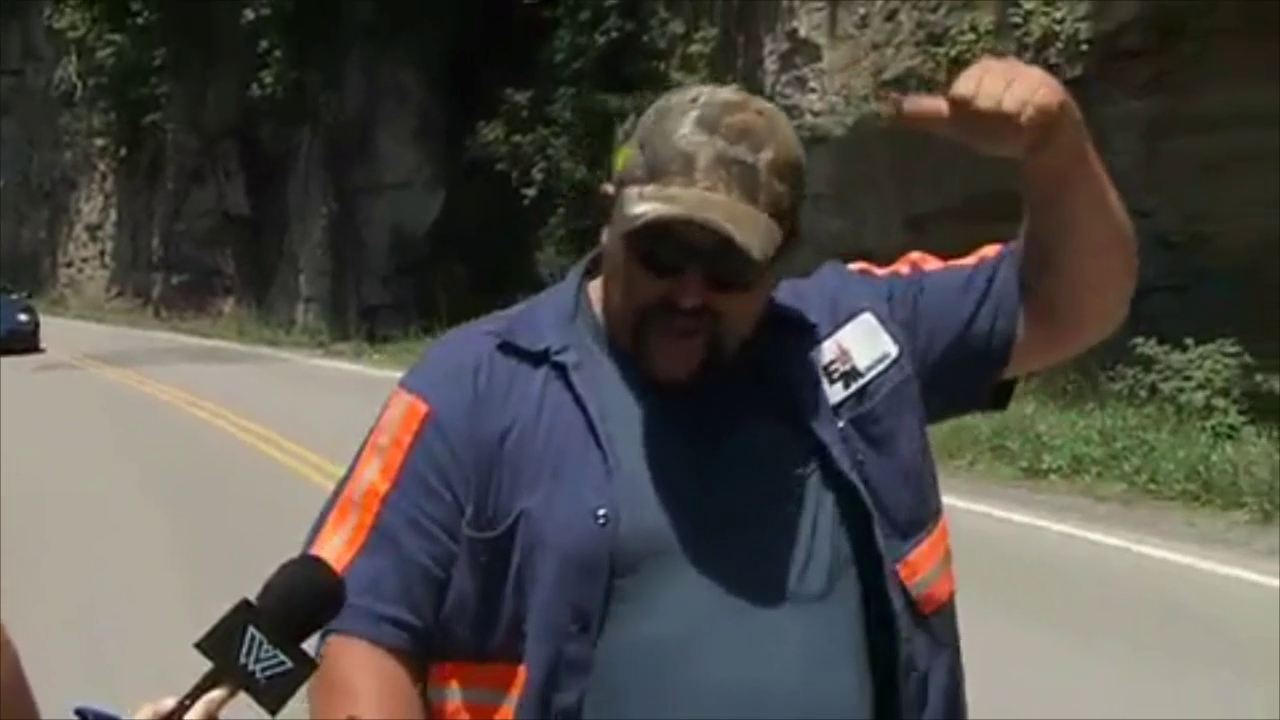
\includegraphics[width=4.2cm]{Figures/mmCult5/frame118.png}  

\end{tabular}
\caption{Cultural Level - Example 5}
\begin{footnotesize}

\end{footnotesize}
\label{fig:figure1}
\end{figure}

\section{Socio-Economic Level}

\subsection{Socio-Economic Level - Example 1}


\begin{footnotesize}

Source: \url{https://www.youtube.com/embed/gU7PBoy-wFE?start=10&end=21}\\
\textit{Embeded videos require Adobe Flash.}
\begin{center}
\includemedia[width=9.60cm,height=5.40cm,activate=pageopen,
passcontext,
transparent,
addresource=Figures/06.mp4,
flashvars={source=Figures/06.mp4}
]{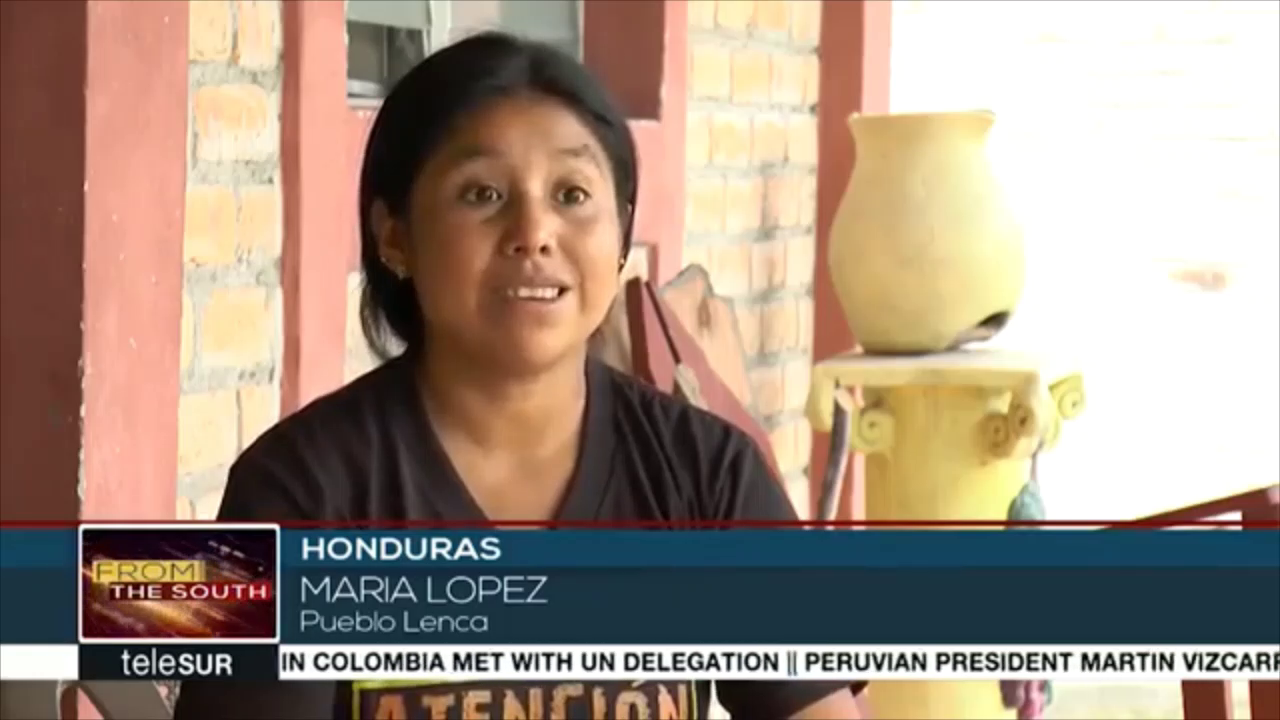
\includegraphics{Figures/mmEcon/frame304.png}}{VPlayer.swf}
\end{center}
\end{footnotesize}

\begin{footnotesize}
\texttt{(Translated from Spanish - only gesture annotation)
The worst impacts have been state violence. Why? Because we have comrades who have been killed following military harassment. [We've already lost one person].\textsuperscript{1}}
\end{footnotesize}

\begin{footnotesize}
\begin{enumerate}
   \item Raised eyebrows; wide eyes; extenuated blinks
\end{enumerate}
\end{footnotesize}

\begin{figure}[H]
\centering
\begin{tabular}{llll}
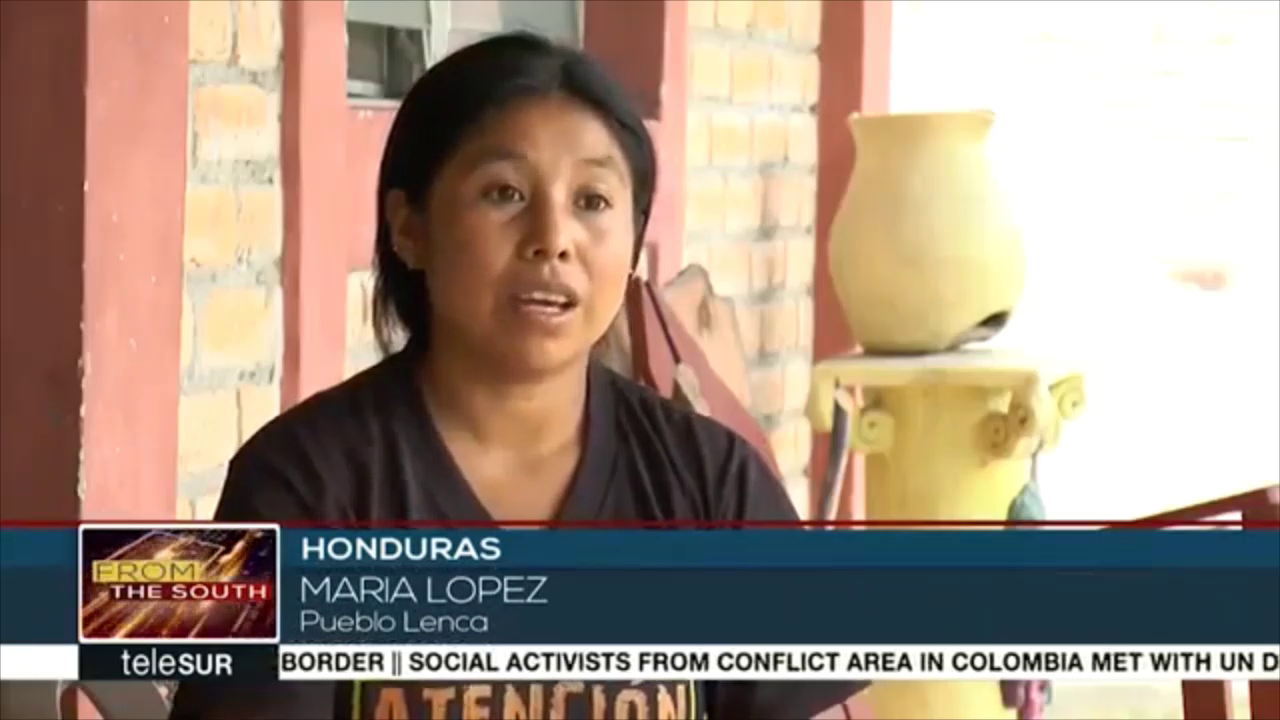
\includegraphics[width=4.2cm]{Figures/mmEcon/frame66.png} & 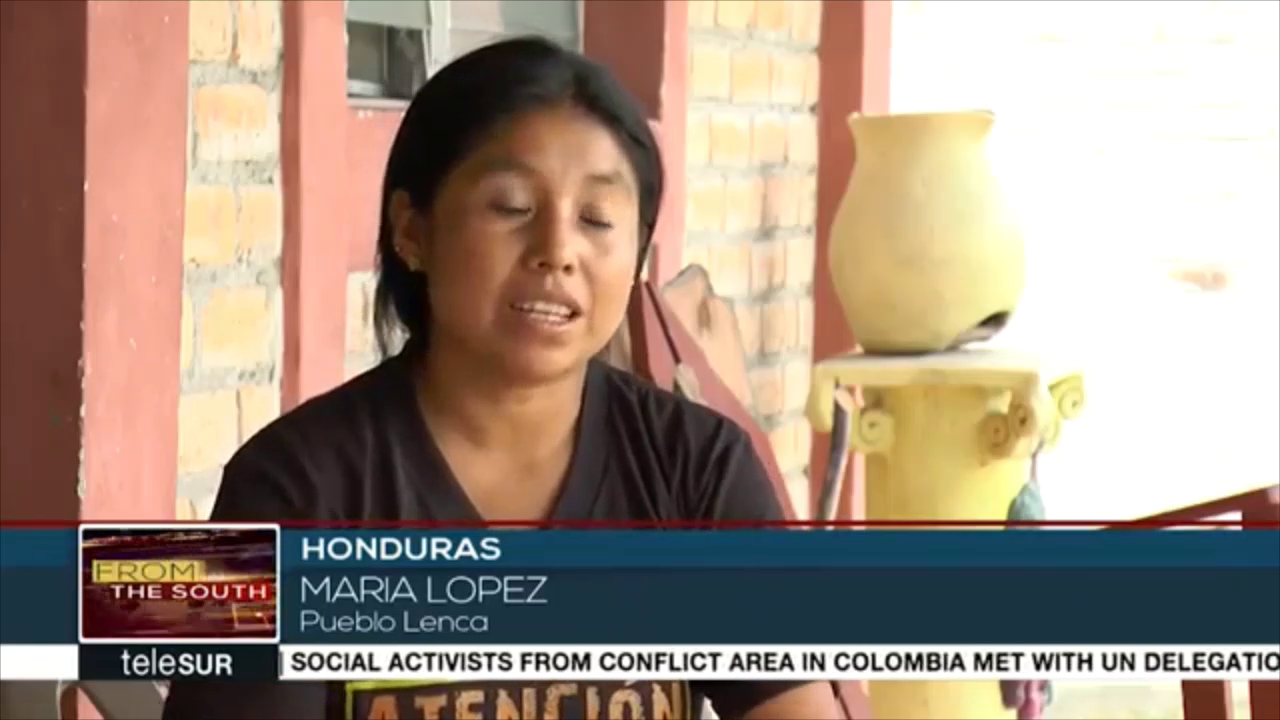
\includegraphics[width=4.2cm]{Figures/mmEcon/frame110.png} & 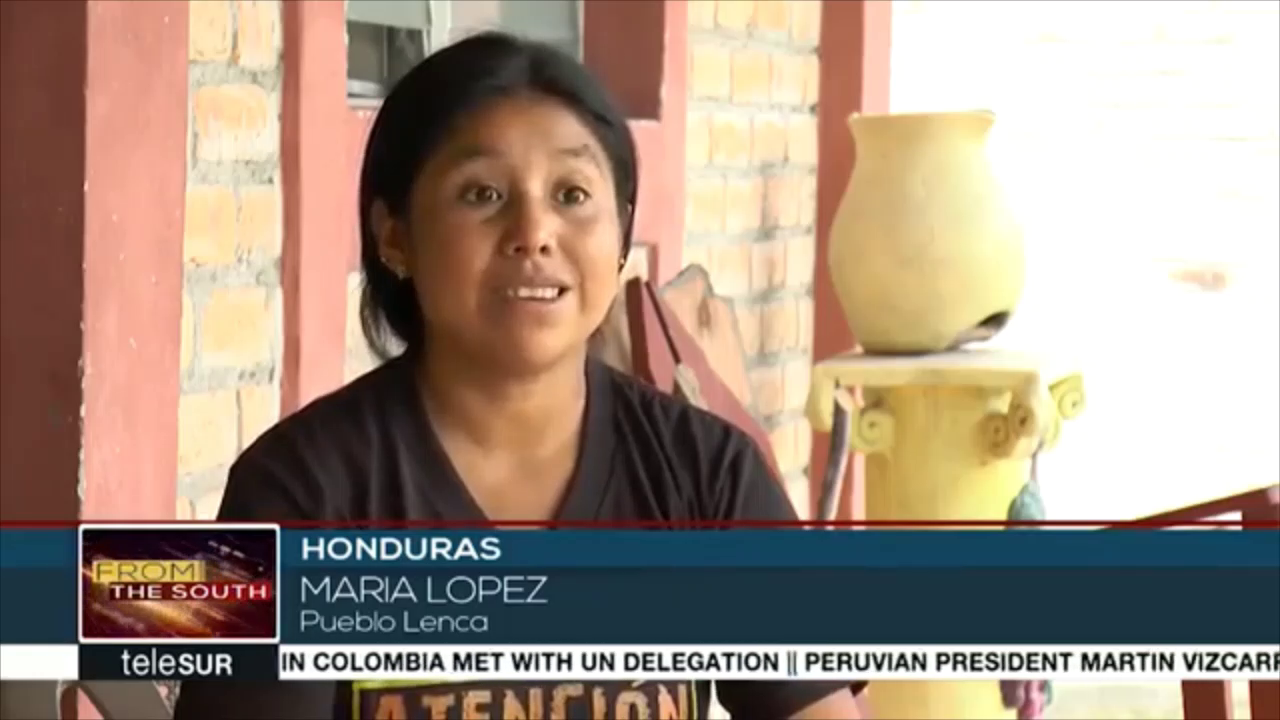
\includegraphics[width=4.2cm]{Figures/mmEcon/frame304.png}  
\end{tabular}
\caption{Socio-Economic level - Example 1}
\begin{footnotesize}

\end{footnotesize}
\label{fig:figure1}
\end{figure}





\subsection{Socio-Economic Level - Example 2}

\begin{footnotesize}
Source: \url{https://www.youtube.com/embed/Sh0_Wf8F4RM?start=390&end=420}\\
\textit{Embeded videos require Adobe Flash.}
\begin{center}
\includemedia[width=9.60cm,height=5.40cm,activate=pageopen,
passcontext,
transparent,
addresource=Figures/11.mp4,
flashvars={source=Figures/11.mp4}
]{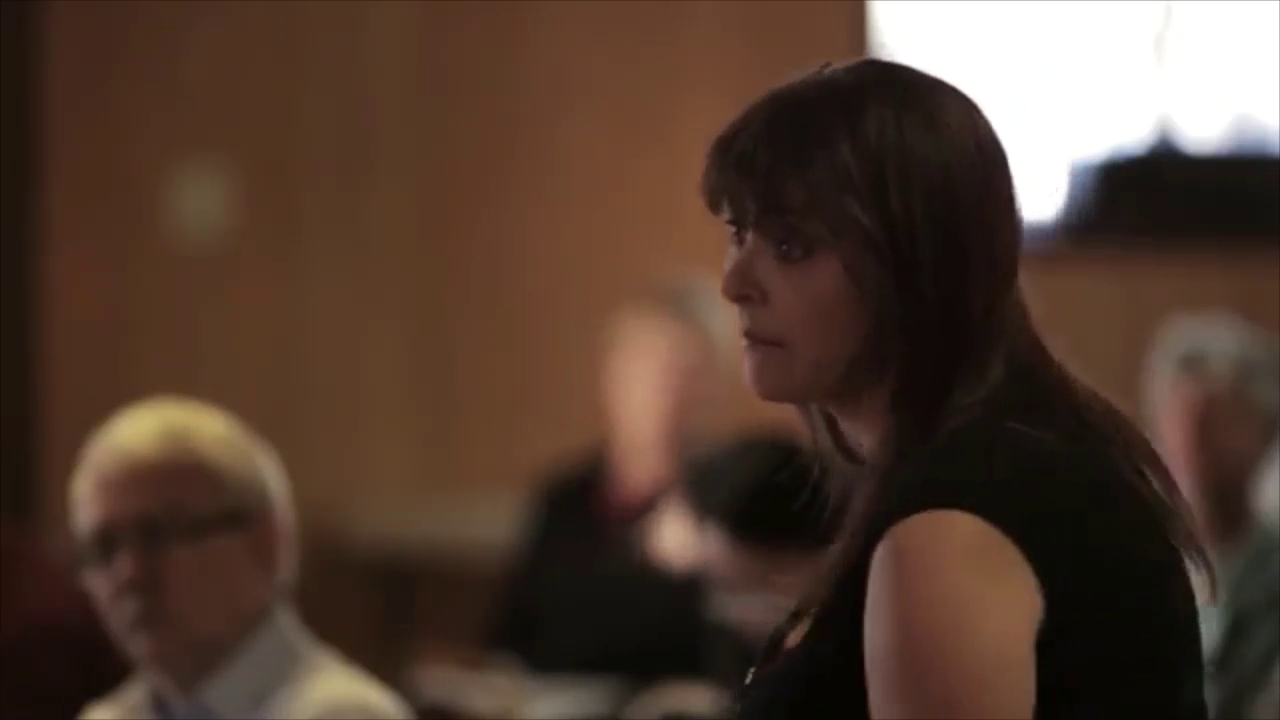
\includegraphics{Figures/mmEcon1/frame988.png}}{VPlayer.swf}
\end{center}
\end{footnotesize}



\begin{footnotesize}

\texttt{<\annotate{Five years} we'e been trying to keep our doors open, \annotate{thinking} (.) any day now> those jobs were going to be here. >These are the only people that have come in and offered us jobs$\uparrow$< If \annotate{any} of the people here who are against it had come in and [said they had jobs to match it, we'd be behind that too. But right now this is all we've got]\textsuperscript{1}. Everyone one of you who has stood up against this could have brought in jobs [for \annotate{us}.]\textsuperscript{2}}
\end{footnotesize}

\begin{footnotesize}
\begin{enumerate}
   \item Raised and upward slanted eyebrows, stressed blink
   \item Hand points inwards toward chest; index finger extended
\end{enumerate}
\end{footnotesize}

\begin{figure}[H]
\centering
\begin{tabular}{llll}
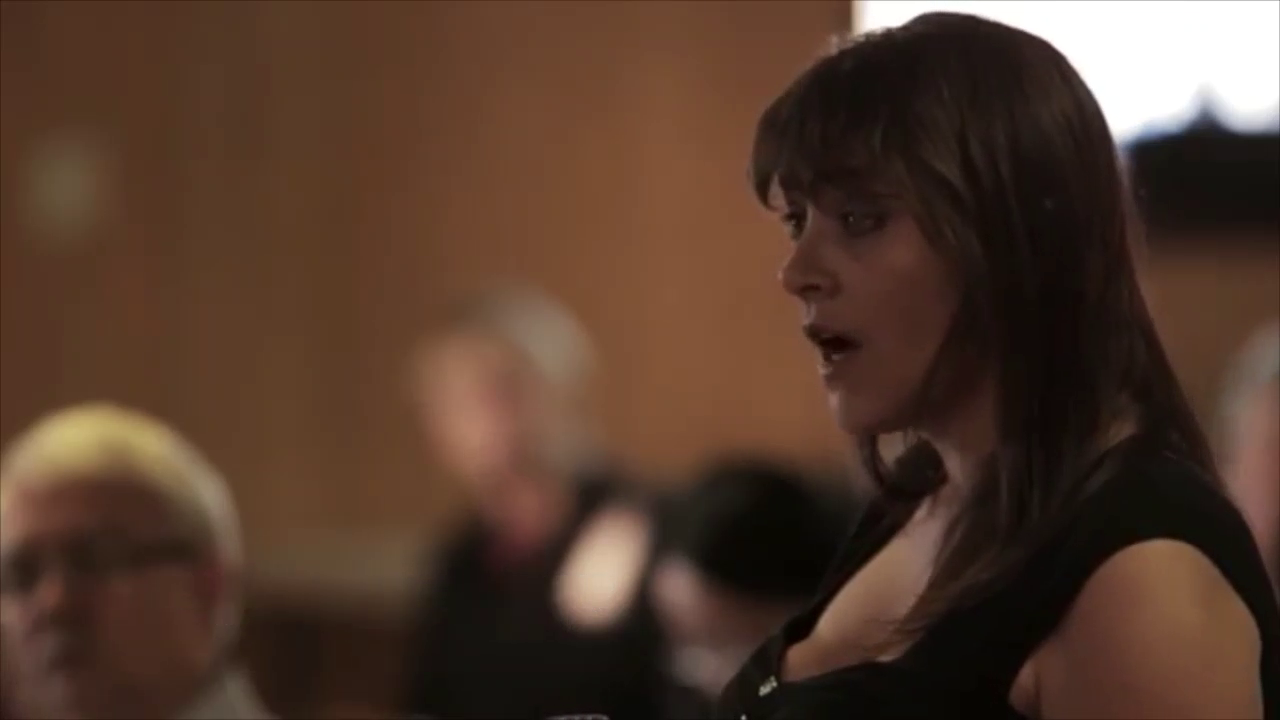
\includegraphics[width=4.2cm]{Figures/mmEcon1/frame413.png} & 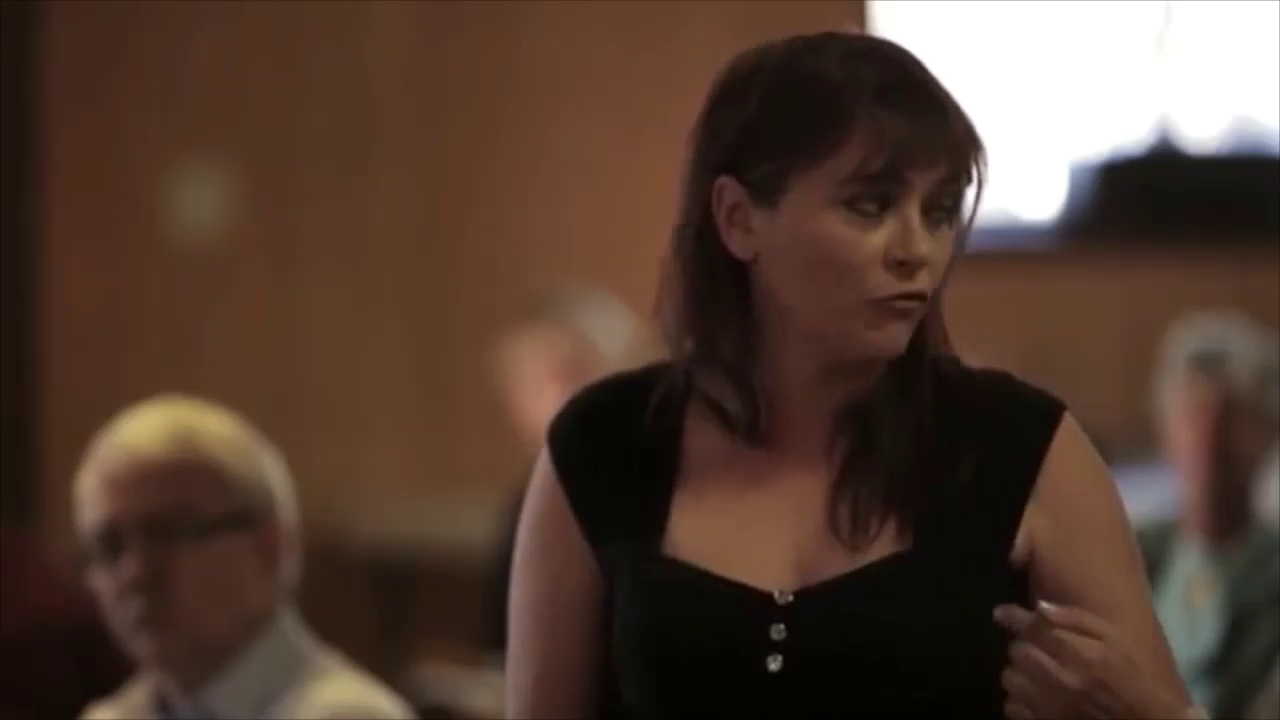
\includegraphics[width=4.2cm]{Figures/mmEcon1/frame725.png} & 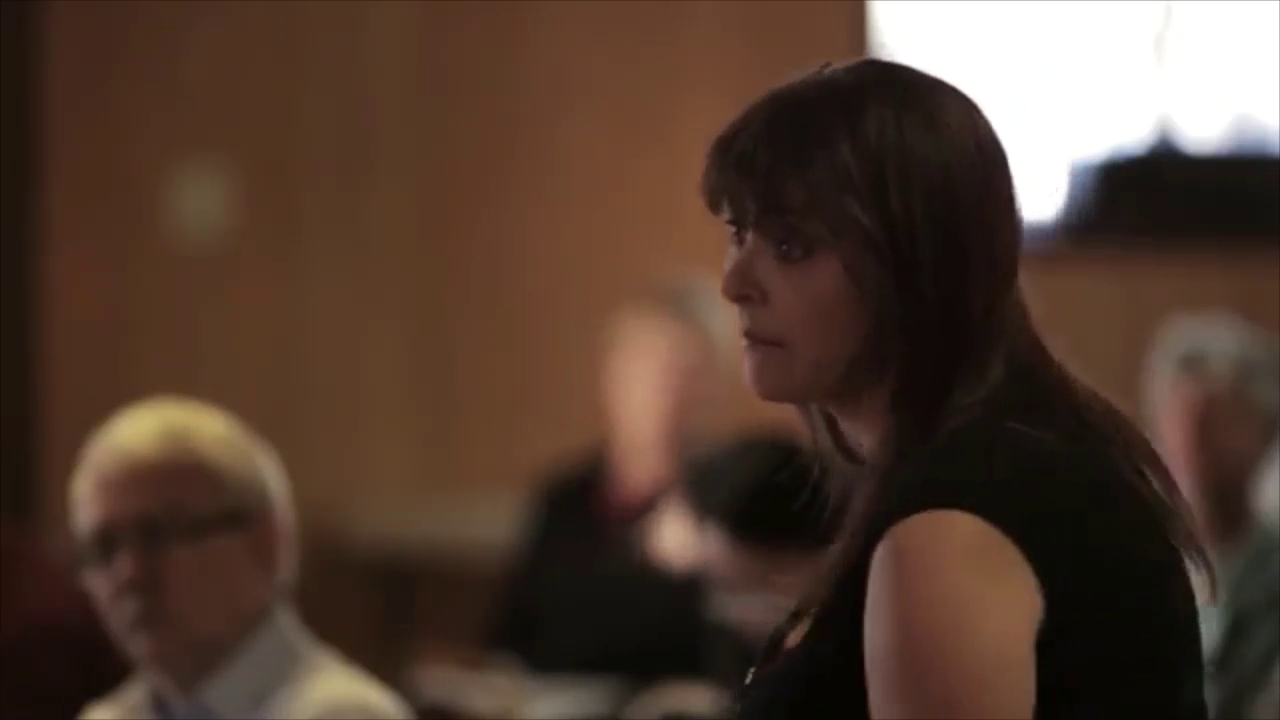
\includegraphics[width=4.2cm]{Figures/mmEcon1/frame988.png}  
\end{tabular}
\caption{Socio-Economic level - Example 2}
\begin{footnotesize}

\end{footnotesize}
\label{fig:figure1}
\end{figure}

\begin{figure}[H]
\centering
\begin{tabular}{llll}
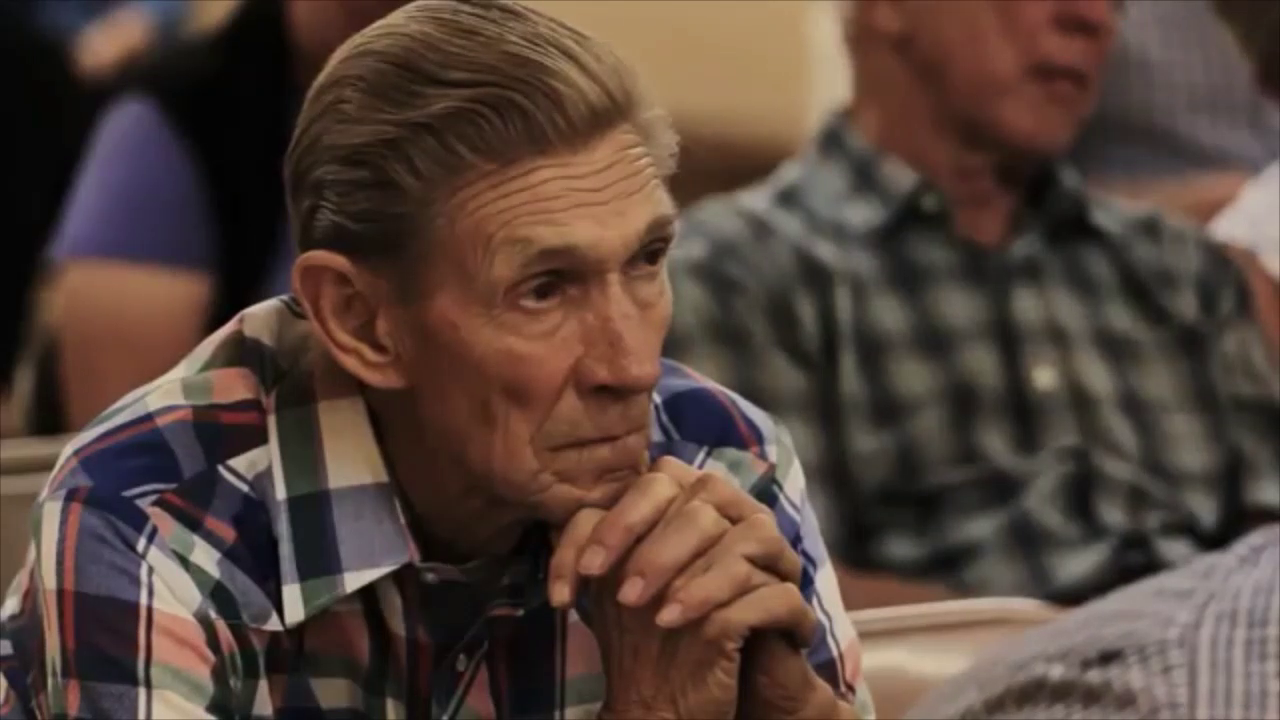
\includegraphics[width=5cm]{Figures/mmEcon2/frame137.png} &  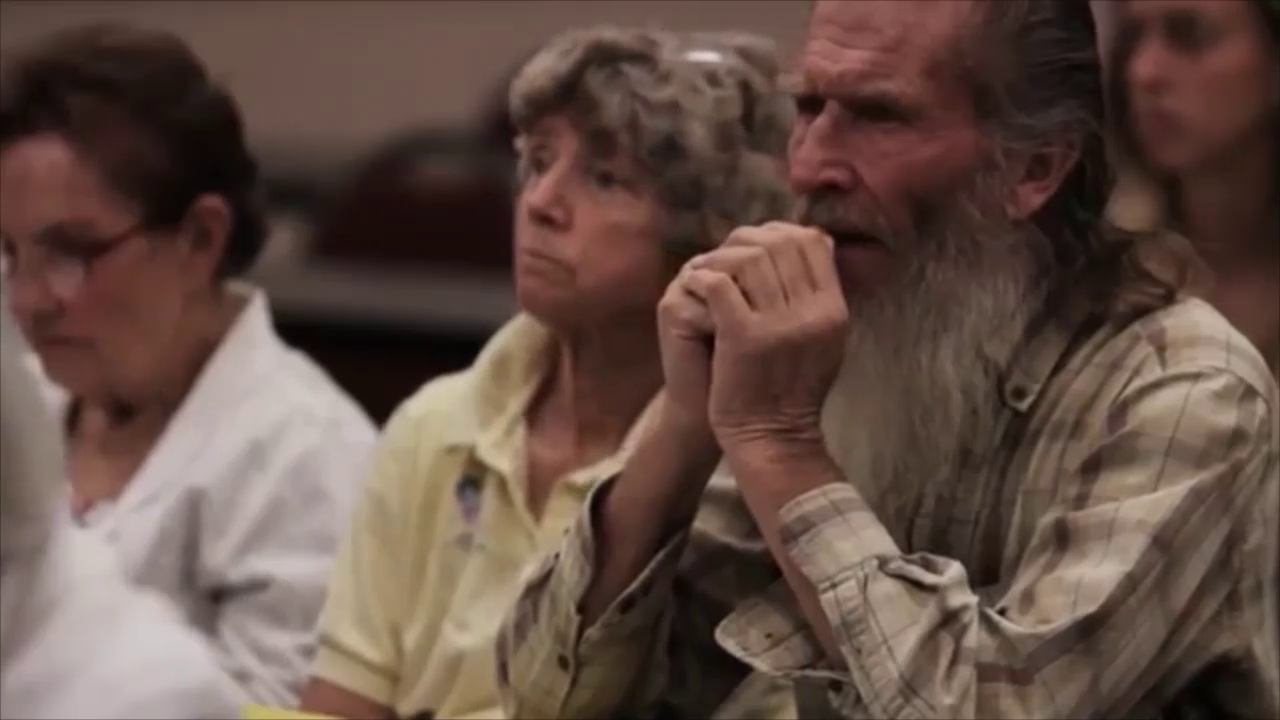
\includegraphics[width=5cm]{Figures/mmEcon2/frame222.png} \\

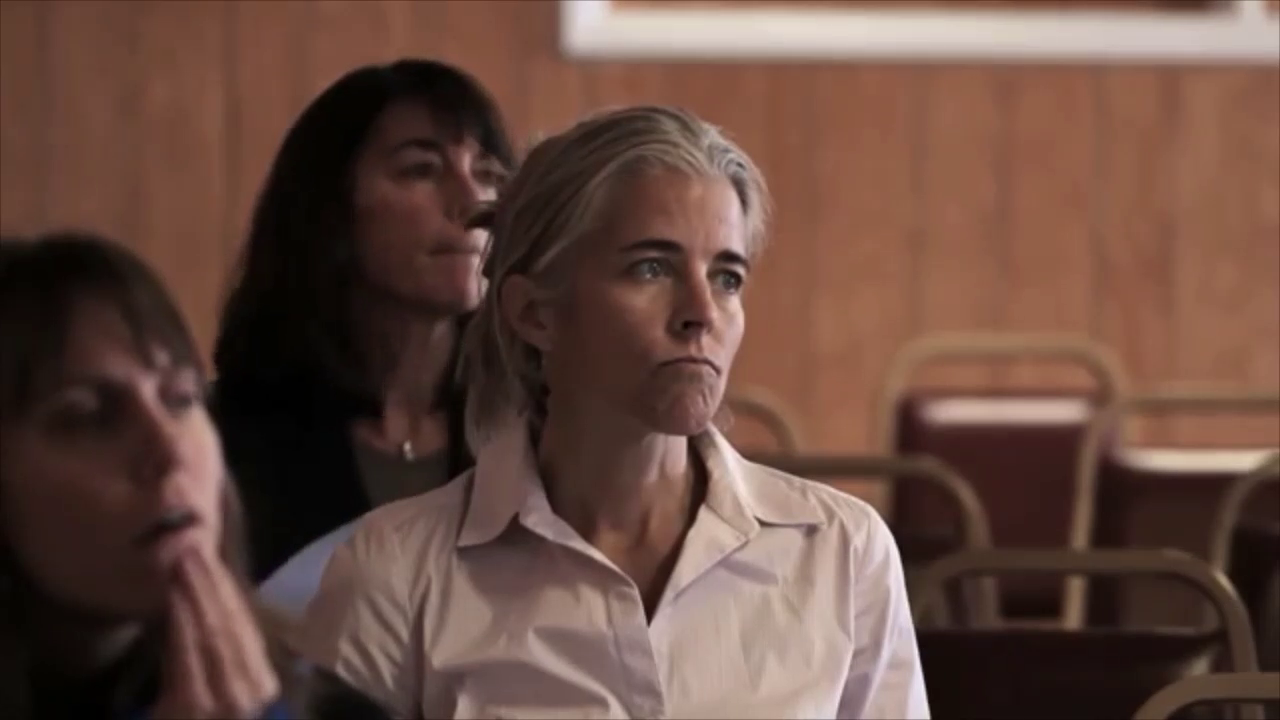
\includegraphics[width=5cm]{Figures/mmEcon2/frame529.png} & 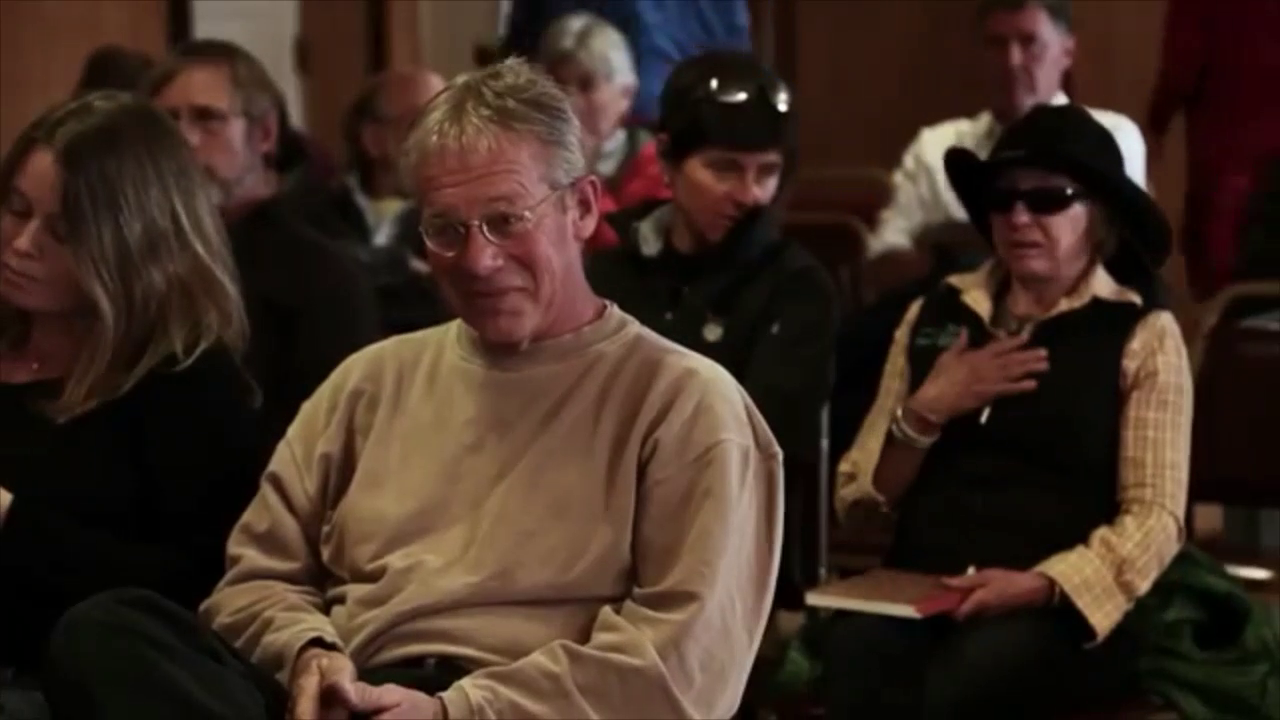
\includegraphics[width=5cm]{Figures/mmEcon2/frame857.png}  

\end{tabular}
\caption{Socio-economic level, listener reactions}
\label{fig:figure1}
\end{figure}




















\subsection{Socio-Economic Level - Example 3}


\begin{footnotesize}

Source: \url{https://www.youtube.com/embed/vBhvFWRLiOs?start=1299&end=1316}\\
\textit{Embeded videos require Adobe Flash.}
\begin{center}
\includemedia[width=9.60cm,height=5.40cm,activate=pageopen,
passcontext,
transparent,
addresource=Figures/19.mp4,
flashvars={source=Figures/19.mp4}
]{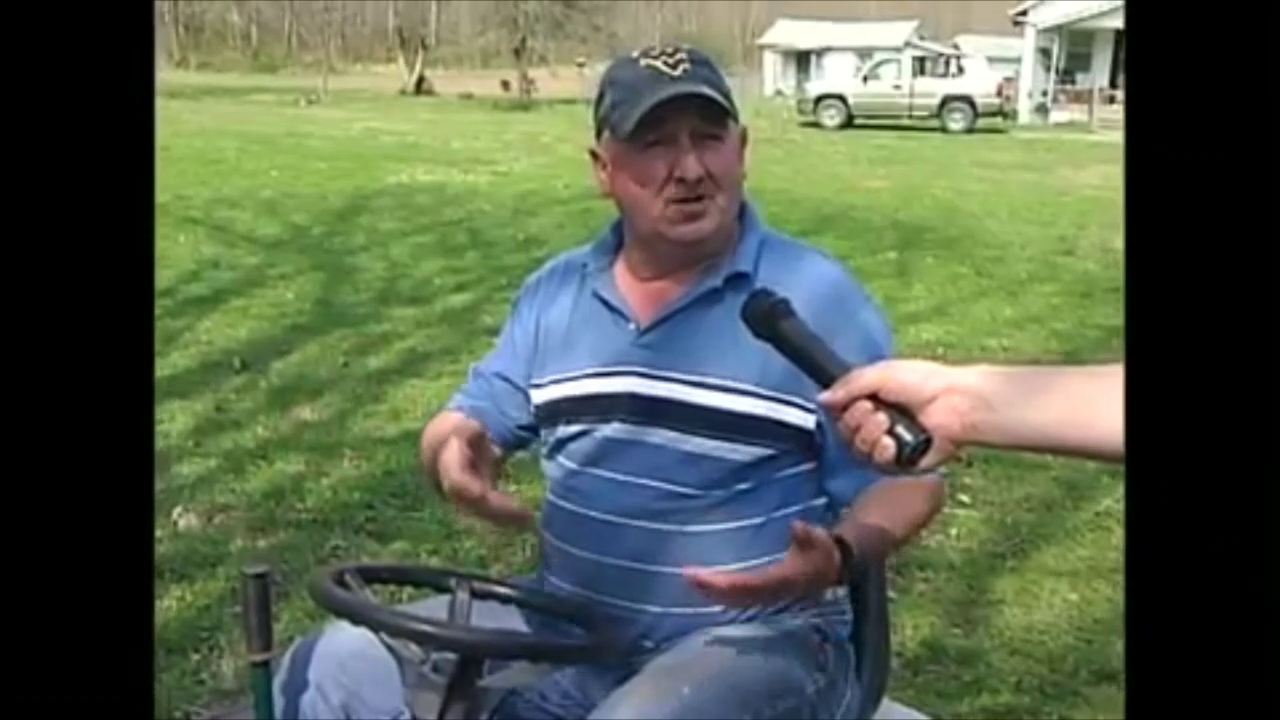
\includegraphics{Figures/mmEcon3/frame610.png}}{VPlayer.swf}
\end{center}
\end{footnotesize}



\begin{footnotesize}
\texttt{[They're fighting]\textsuperscript{1} a losing battle I feel (.) myself I feel like they're just fighting a losing battle, because the <[\annotate{politicians}]\textsuperscript{2} and the [\annotate{big} coal companies and things> \annotate{they're} going to win hands down >because the judges and arbitrators are just going to go their way.<]\textsuperscript{3} }
\end{footnotesize}

\begin{footnotesize}
\begin{enumerate}
   \item Both hands extend outward, palms up
   \item Both hands motion forward/downward, palms down
   \item Both hands extend outward, palms up, with emphasis
\end{enumerate}
\end{footnotesize}

\begin{figure}[H]
\centering
\begin{tabular}{llll}
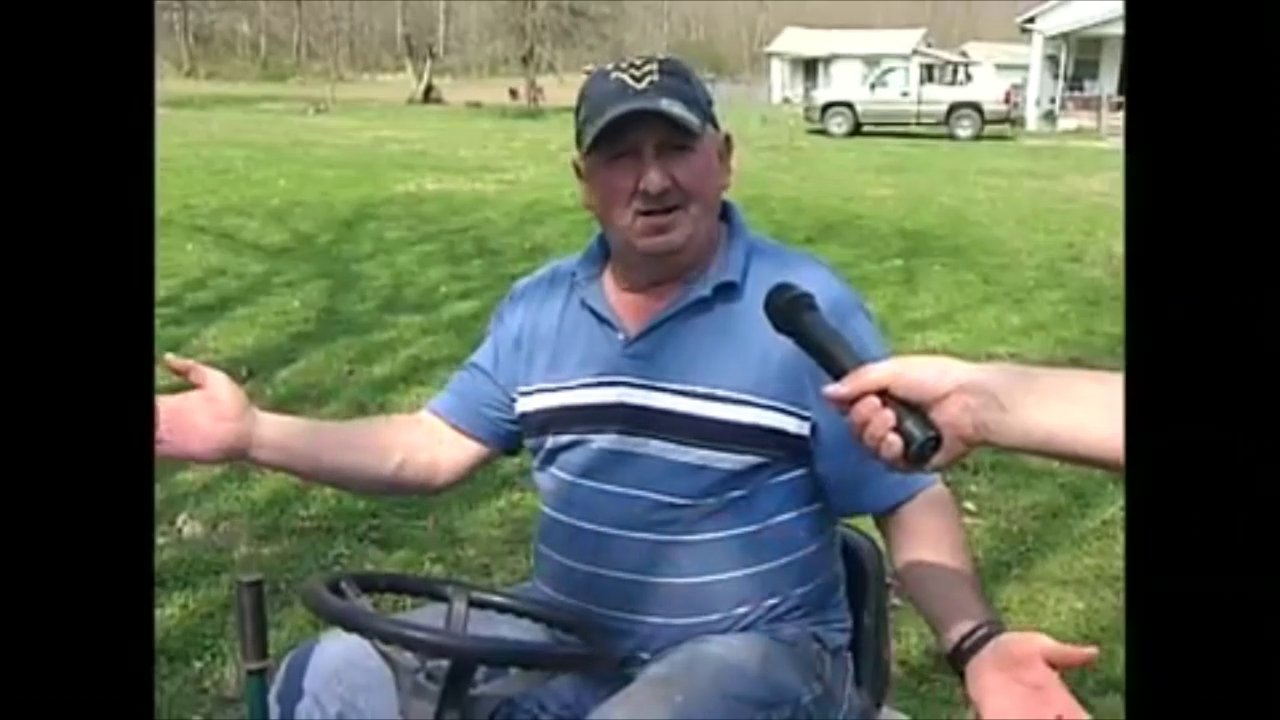
\includegraphics[width=4.2cm]{Figures/mmEcon3/frame189.png} & 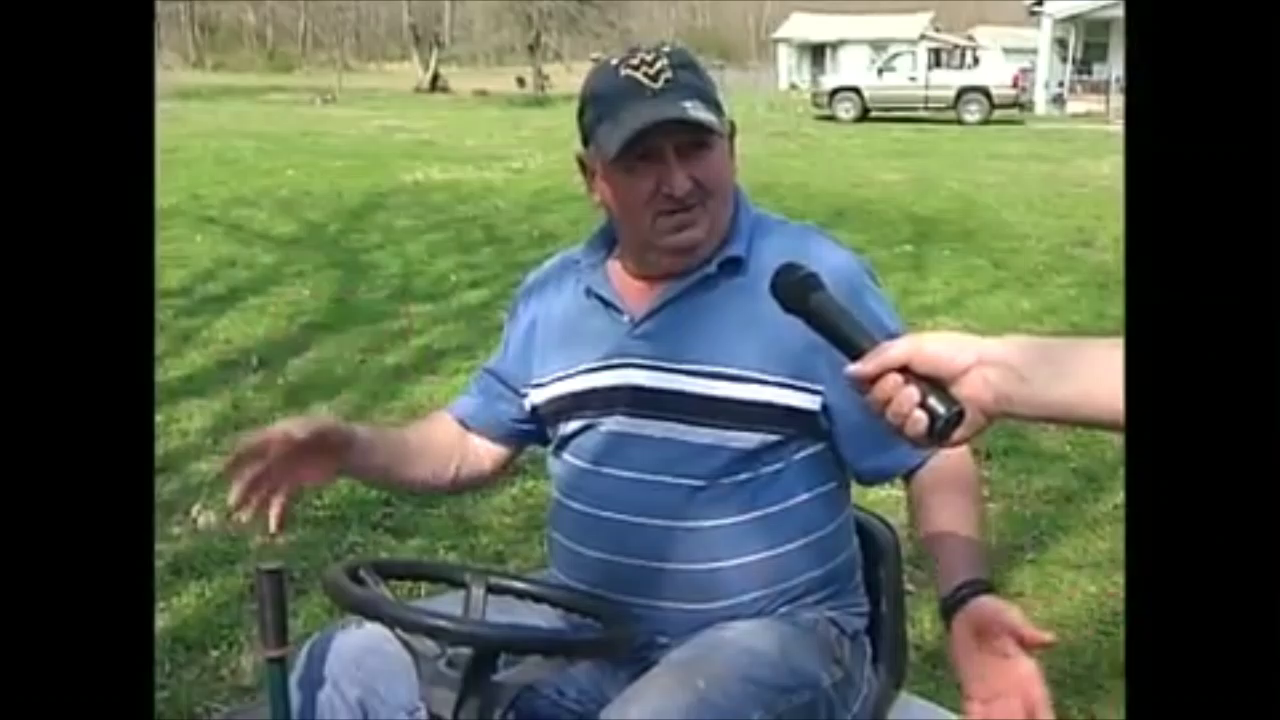
\includegraphics[width=4.2cm]{Figures/mmEcon3/frame450.png} & 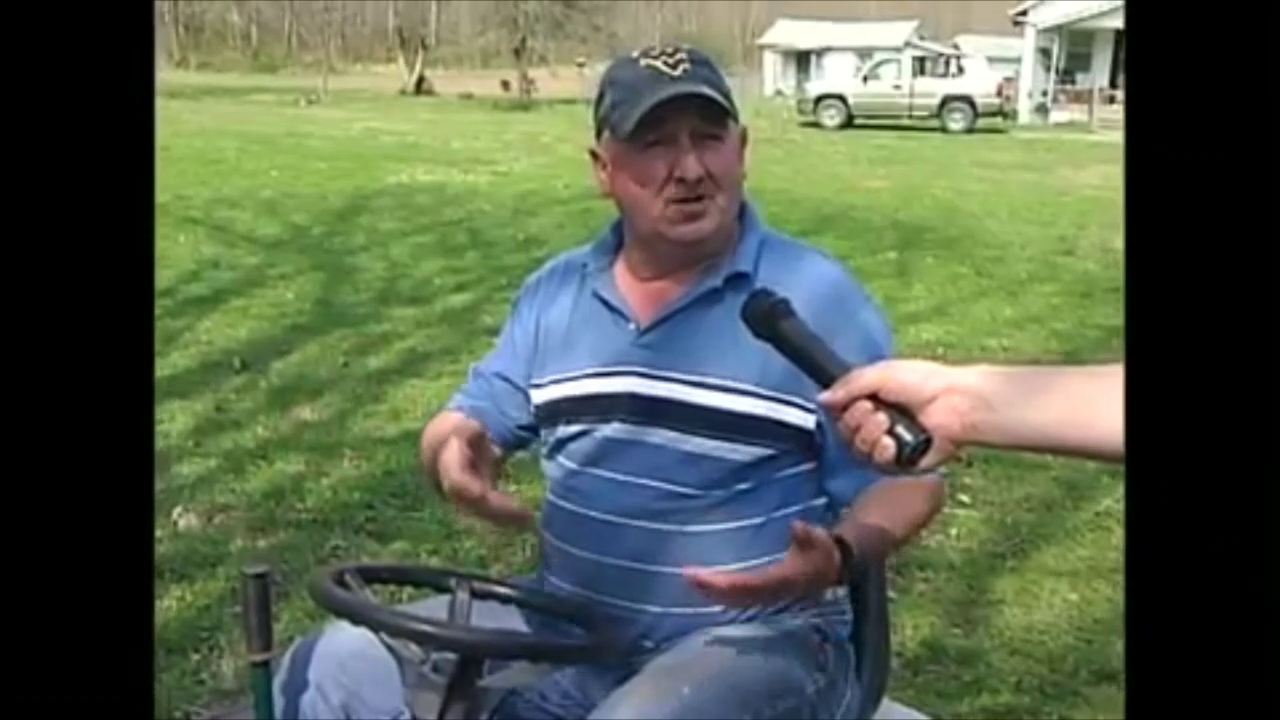
\includegraphics[width=4.2cm]{Figures/mmEcon3/frame610.png}  
\end{tabular}
\caption{Socio-Economic Level - Example 3}
\begin{footnotesize}

\end{footnotesize}
\label{fig:figure1}
\end{figure}









\subsection{Socio-Economic Level - Example 4}

\begin{footnotesize}

Source: \url{https://www.youtube.com/embed/vBhvFWRLiOs?start=58&end=75}\\
\textit{Embeded videos require Adobe Flash.}
\begin{center}
\includemedia[width=9.60cm,height=5.40cm,activate=pageopen,
passcontext,
transparent,
addresource=Figures/16.mp4,
flashvars={source=Figures/16.mp4}
]{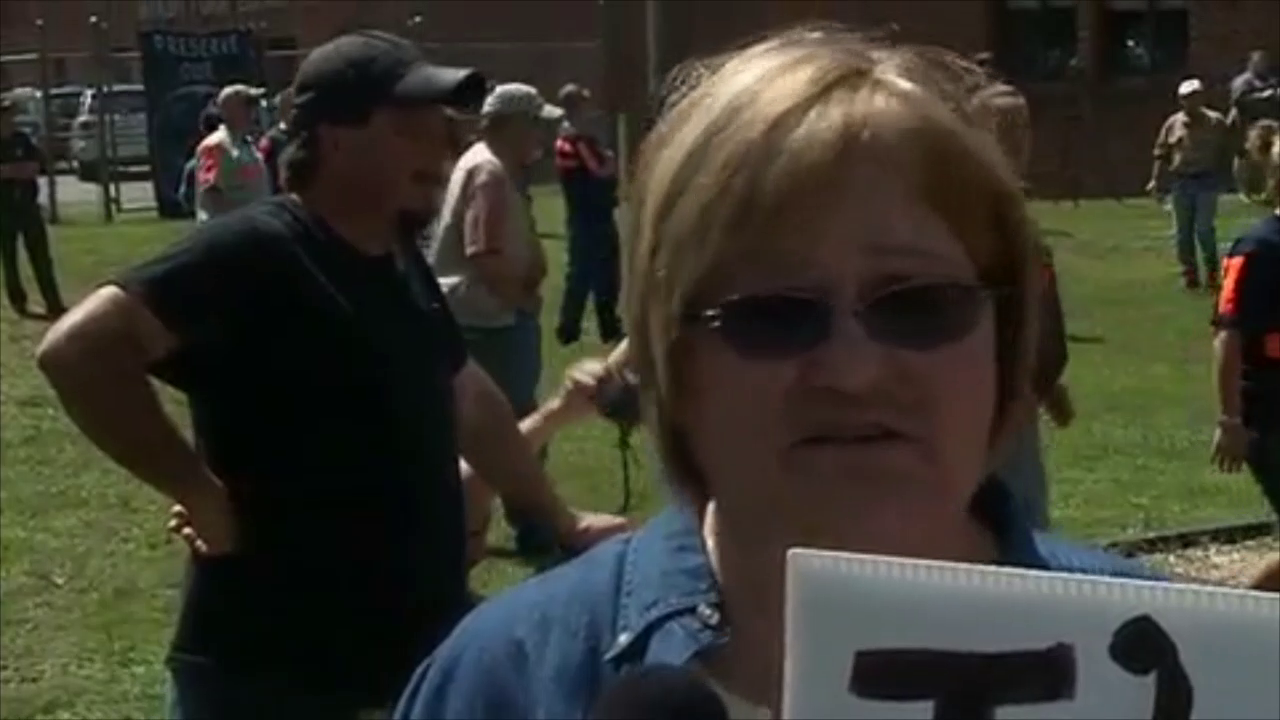
\includegraphics{Figures/mmEcon4/frame3.png}}{VPlayer.swf}
\end{center}
\end{footnotesize}


\begin{footnotesize}
\texttt{If you choose to live in West Virginia, [this is (.) this is the best paying job there is$\uparrow$]\textsuperscript{1}. \textit{Interviewer}: What happens if mountain top removal goes away, what happens to you and your family? \annotate{WE GO HUNGRY!}\textsuperscript{2}}

\end{footnotesize}

\begin{footnotesize}
\begin{enumerate}
   \item Shoulders raise; nodding
   \item Eyebrows raise
\end{enumerate}
\end{footnotesize}

\begin{figure}[H]
\centering
\begin{tabular}{llll}
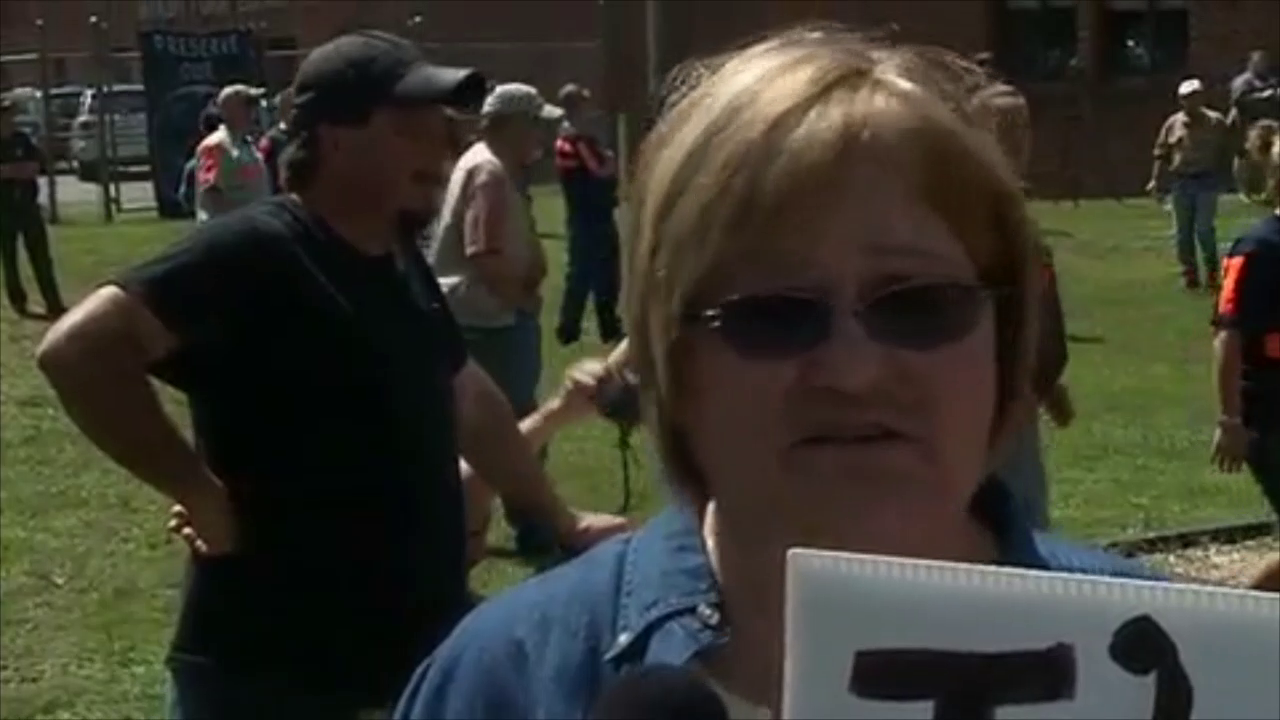
\includegraphics[width=4.2cm]{Figures/mmEcon4/frame3.png} & 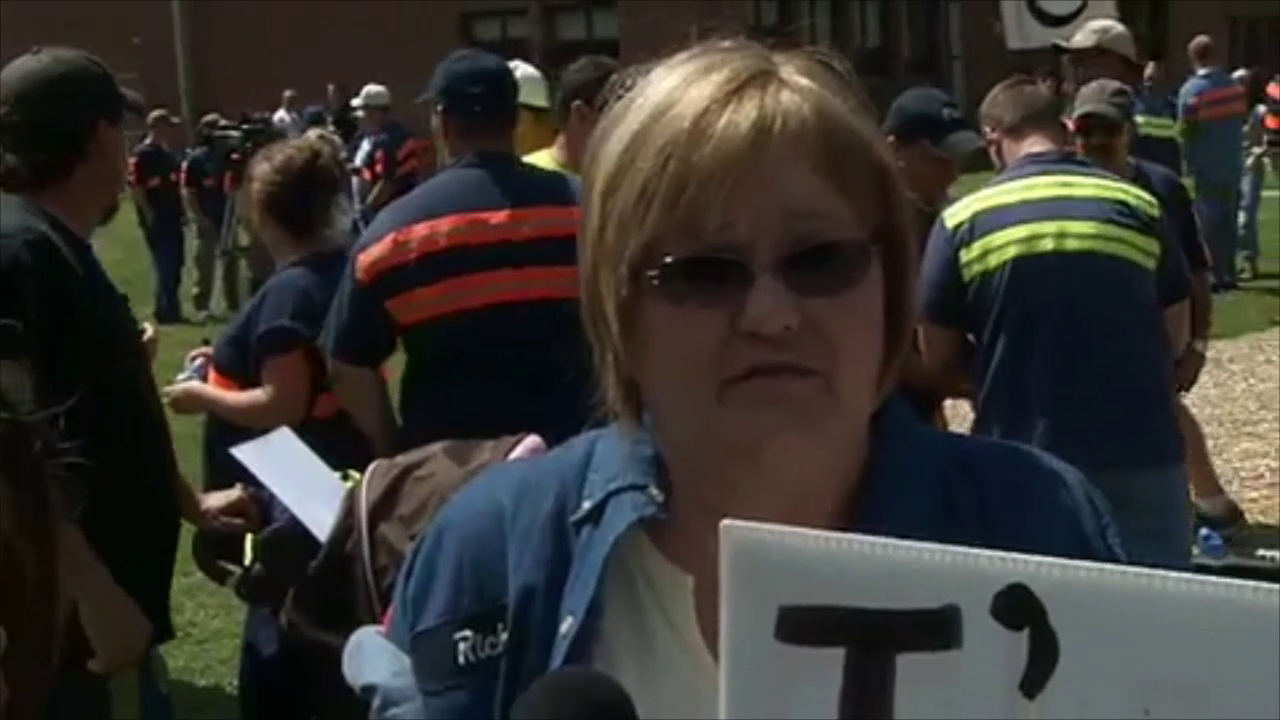
\includegraphics[width=4.2cm]{Figures/mmEcon4/frame551.png} & 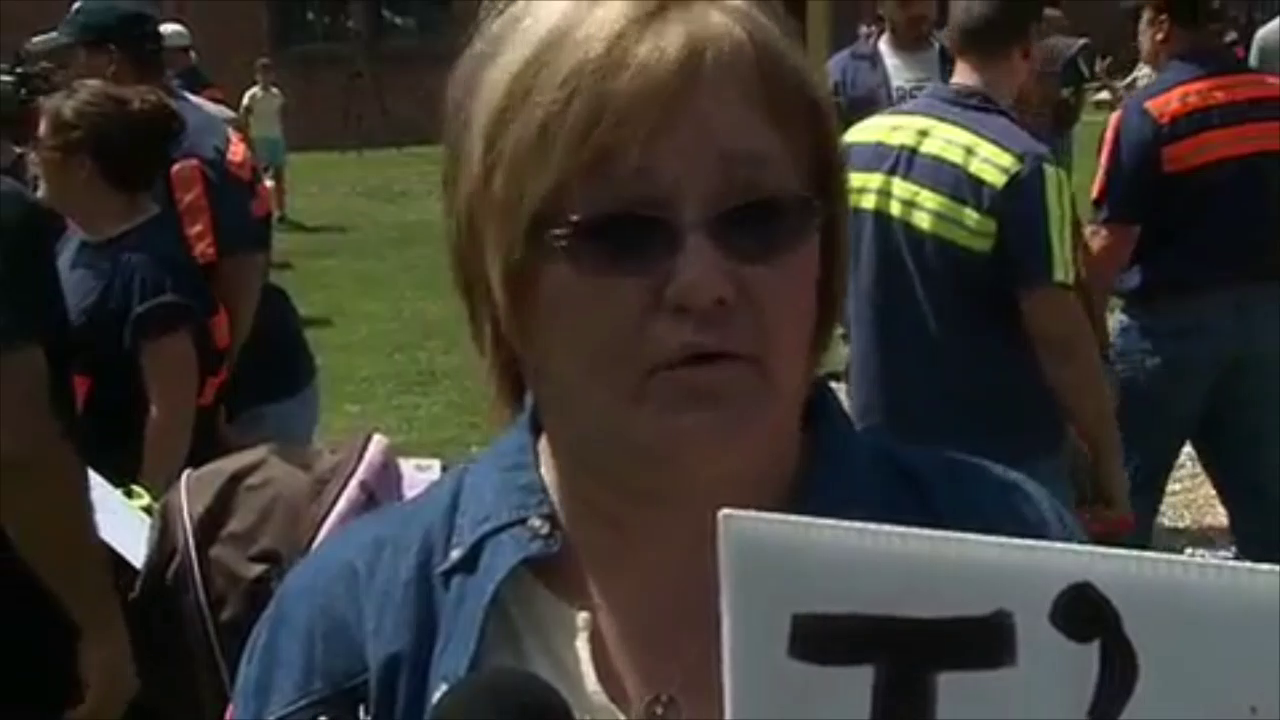
\includegraphics[width=4.2cm]{Figures/mmEcon4/frame901.png}  
\end{tabular}
\caption{Socio-Economic level - Example 4}
\begin{footnotesize}

\end{footnotesize}
\label{fig:figure1}
\end{figure}